% Computer Vision Course Final Project Report — CVPR 2026 layout (Task 1 + Task 2)
\documentclass[10pt,twocolumn,letterpaper]{article}

\setcounter{secnumdepth}{3}
\usepackage{fontspec}
\setmainfont{Times New Roman}[
  BoldFont = Times New Roman Bold,
  ItalicFont = Times New Roman Italic,
  BoldItalicFont = Times New Roman Bold Italic
]
\newfontfamily\cvprboldfont[
  Path=/System/Library/Fonts/Supplemental/,
  Extension=.ttf,
  UprightFont=Times New Roman Bold,
  BoldFont=Times New Roman Bold,
  ItalicFont=Times New Roman Bold Italic,
  BoldItalicFont=Times New Roman Bold Italic,
]{}

\usepackage[pagenumbers]{./author-kit-CVPR2026-v1-latex-/cvpr}
\setlength{\parindent}{0pt}
\renewcommand{\partname}{Part}
\makeatletter
\renewcommand\@part[2][]{%
  \ifnum \c@secnumdepth >-2\relax
    \refstepcounter{part}%
    \addcontentsline{toc}{part}{\thepart\hspace{1em}#2}%
  \else
    \addcontentsline{toc}{part}{#2}%
  \fi
  \markboth{}{\partname~\thepart\ #2}%
  \vspace{0.4em}%
  \noindent{\bfseries\large \partname~\thepart\quad #2\par}%
  \vspace{0.25em}%
}
\makeatother
\usepackage{enumitem}
\usepackage[english]{babel}
\usepackage{microtype}
\microtypesetup{protrusion=true}
\setlength{\emergencystretch}{2.5em}
\tolerance=3500
\pretolerance=200
\raggedbottom
\setlength{\parskip}{0pt plus 0pt minus 0pt}
\usepackage{array}
\usepackage{ragged2e}
\usepackage{adjustbox}
\usepackage{graphicx}
\usepackage{subcaption}
\usepackage{float}
\usepackage{stfloats}
\newcounter{apptab}
\renewcommand{\theapptab}{\arabic{apptab}}
\newcommand{\apptabcaption}[2]{%
  \refstepcounter{apptab}%
  \label{#1}%
  \vspace{\abovecaptionskip}%
  {\footnotesize\bfseries Supplementary Table~\theapptab: #2\par}%
  \vspace{\belowcaptionskip}%
}
\newcommand{\apptabref}[1]{\hyperref[#1]{Supplementary Table~\ref*{#1}}}
\newcommand{\tabref}[1]{Table~\ref{#1}}
\newcommand{\tablenote}[1]{\par\vspace{0.15em}{\footnotesize #1}}
\newcommand{\tbd}{[TBD]}
\usepackage{listings}
\lstset{
  basicstyle=\ttfamily\scriptsize,
  breaklines=true,
  columns=fullflexible,
  frame=single,
  framesep=3pt,
  xleftmargin=0pt,
  xrightmargin=0pt
}

\setlist{nosep,leftmargin=*}
\setlength{\textfloatsep}{6pt plus 2pt minus 2pt}
\setlength{\floatsep}{4pt plus 2pt minus 2pt}
\setlength{\intextsep}{4pt plus 2pt minus 2pt}
\setlength{\abovecaptionskip}{2pt}
\setlength{\belowcaptionskip}{0pt}
\setlength{\abovedisplayskip}{4pt plus 2pt minus 2pt}
\setlength{\belowdisplayskip}{4pt plus 2pt minus 2pt}

\definecolor{cvprblue}{rgb}{0.21,0.49,0.74}
\usepackage[breaklinks,colorlinks,allcolors=cvprblue]{hyperref}
\renewcommand{\tablename}{Table}

\makeatletter
\renewcommand\@maketitle{%
   \newpage
   \null
   \iftoggle{cvprrebuttal}{\vspace*{-.3in}}{\vskip .375in}
   \begin{center}
      \iftoggle{cvprrebuttal}{%
        {\large\@title\par}%
      }{%
        {\Large\@title\par}%
      }%
      \iftoggle{cvprrebuttal}{\vspace*{-22pt}}{\vspace*{24pt}}{%
        \large
        \lineskip .5em
        \begin{tabular}[t]{c}
          \iftoggle{cvprfinal}{%
            \@author
          }{%
            \iftoggle{cvprrebuttal}{}{%
              Anonymous \confName~submission\\
              \vspace*{1pt}\\
              Paper ID \paperID
            }%
          }%
        \end{tabular}
        \par
      }%
      \vskip .5em
      \vspace*{12pt}
   \end{center}
}
\def\abstract{%
   \iftoggle{cvprpagenumbers}{}{%
     \thispagestyle{empty}
   }%
   \begin{center}%
     {\large\cvprboldfont Abstract}%
   \end{center}%
   \vspace*{12pt}\noindent%
   \it\ignorespaces%
}
\makeatother

\def\paperID{*****}
\def\confName{CVPR}
\def\confYear{2026}

\title{{\cvprboldfont Multi-Object 3D Reconstruction and Cross-Environment Generalization of Embodied Policies}}

\author{%
  Liesen Gai \quad 23307130013@m.fudan.edu.cn\\[0.25em]
  \textit{Both Task 1 and Task 2 were completed independently by the author.}\\[0.25em]
}

\begin{document}
\maketitle

\begin{abstract}
This paper presents experimental studies on two core tasks: multi-source 3D asset generation and scene fusion, and cross-environment generalization of embodied intelligence policies.
For 3D generation and fusion, three heterogeneous pipelines---multi-view 2DGS reconstruction, text-driven SDS generation, and single-image Magic123 generation---build three asset types, with fusion rendering in real scenes achieved via a unified mesh representation. Experiments confirm that multi-view reconstruction, with 36-view photometric constraints, reaches 36.12\,dB novel-view rendering accuracy with a core pipeline time of only 542\,s, offering optimal precision and efficiency; pure text generation exhibits inherent Janus topology defects, and extending training steps cannot break the geometric identifiability ceiling; single-image generation can anchor front-view accuracy, but back structure is affected by symmetry bias in generative priors. The quality ceiling of the three paradigms is determined by the dimension and determinism of supervision signals; diffusion backpropagation accounts for 74.0\% of total core compute time, and the cost-effectiveness of adding real observations far exceeds stacking generative training iterations.
For embodied policy generalization, using the ACT action-chunking algorithm in the LeRobot framework, we compare zero-shot cross-domain performance between single-environment and three-environment joint training. Results show that single-environment training yields lower in-distribution error, but the generalization gap reaches 0.212 when transferring to unseen environment~D; multi-environment joint training trades a small in-distribution precision loss to reduce the generalization gap by 66\% and raise task success rate by 10.3 percentage points. Mechanism analysis shows that visual distribution shift only parallel-shifts the error baseline of action chunks without changing the degradation rate of error with step index; generalization gains stem from domain-invariant feature extraction by the visual encoder and are unrelated to action temporal modeling.
\end{abstract}

\noindent\textbf{Keywords:} 2D Gaussian Splatting; Score Distillation Sampling; multi-source 3D scene fusion; ACT action-chunking policy; zero-shot cross-environment generalization
\vspace{0.2em}

\part{Multi-Object 3D Reconstruction and AIGC Scene Fusion}

%==============================================================================
\section{Introduction}
\label{sec:t1-intro}
%==============================================================================

\subsection{Background and Motivation}

3D scene understanding is a central problem in computer vision and graphics: recovering object geometry and appearance from multi-view or single-view observations and fusing them with real or synthetic backgrounds in a unified coordinate frame underpins digital twins, virtual reality, and AIGC content production. Traditional multi-view stereo (MVS) pipelines rely on feature matching and dense reconstruction\cite{schoenberger2016sfm,schoenberger2016mvs} and remain engineering-reliable on texture-rich objects with sufficient view coverage; neural radiance fields (NeRF)\cite{mildenhall2020nerf} and accelerated variants such as Instant-NGP\cite{muller2022instantngp} and anti-aliased Mip-NeRF\cite{barron2021mipnerf,barron2022mipnerf360} achieve high-quality novel-view synthesis via differentiable rendering. Recently, 3D Gaussian Splatting\cite{kerbl2023gaussians} and 2D Gaussian Splatting\cite{huang20242dgs} explicitize scene representation, enabling real-time rendering while facilitating mesh and PLY export, which suits multi-source asset generation and scene fusion applications.

Meanwhile, generative 3D content (AIGC-3D) has risen rapidly: Score Distillation Sampling (SDS)\cite{poole2022dreamfusion} distills score functions from pretrained 2D diffusion models\cite{rombach2022ldm} into NeRF or mesh representations for text-to-3D; Magic3D\cite{lin2023magic3d} and ProlificDreamer\cite{wang2023prolificdreamer} continue to improve resolution and diversity. For single-view real objects with only one photograph, Magic123\cite{qian2023magic123} combines 2D diffusion with Zero-1-to-3\cite{liu2023zero123} multi-view priors in a coarse-to-fine two-stage optimization that balances geometric consistency and texture detail. The unified threestudio\cite{threestudio2023} framework lowers the engineering barrier to reproducing DreamFusion-class pipelines.

This report unifies three typical input paradigms: self-captured multi-view real Object~A, text-only virtual Object~B, and single-view real Object~C, with the Mip-NeRF 360\cite{barron2022mipnerf360} public scene as background, completing 2DGS reconstruction and Blender scene fusion. This design forces method selection between ``traditional SfM + explicit Gaussians'' and ``diffusion priors + neural/mesh optimization,'' and engineering integration across heterogeneous pipelines in asset format, scale, and material.

\subsection{Related Work}

\subsubsection{Multi-View Geometry and COLMAP}

Structure-from-Motion (SfM) estimates camera poses and sparse point clouds from unordered image sets; Multi-View Stereo (MVS) further recovers dense depth. COLMAP\cite{schoenberger2016sfm,schoenberger2016mvs} integrates feature extraction, matching, incremental reconstruction, and dense fusion into an open-source toolchain and serves as the de facto camera-calibration frontend for the NeRF/Gaussian splatting community. For Object~A we use COLMAP for SIFT feature matching and incremental pose estimation, providing geometrically consistent camera parameters for subsequent 2DGS.

\subsubsection{Neural Radiance Fields and Explicit Gaussian Splatting}

NeRF\cite{mildenhall2020nerf} encodes a 5D radiance field with an MLP and obtains photorealistic novel views via volume rendering; Mip-NeRF\cite{barron2021mipnerf} and Mip-NeRF 360\cite{barron2022mipnerf360} introduce multi-scale cone sampling to mitigate aliasing and extend to unbounded outdoor scenes. Instant-NGP\cite{muller2022instantngp} accelerates training with hash encoding. 3D Gaussian Splatting\cite{kerbl2023gaussians} uses anisotropic 3D Gaussians with differentiable splatting for real-time rendering; 2D Gaussian Splatting\cite{huang20242dgs} constrains primitives to 2D disk surfels, emphasizing geometrically accurate surface reconstruction and TSDF-fusion export, making trained results easier to convert to editable meshes. We use 2DGS for both Object~A and the background scene.

\subsubsection{Score Distillation and Text-to-3D}

DreamFusion\cite{poole2022dreamfusion} proposes SDS: at randomly sampled render views, pretrained diffusion models apply score-matching gradients to rendered images, optimizing NeRF without 3D training data. Magic3D\cite{lin2023magic3d} introduces coarse-to-fine two-stage training with normal/depth regularization; ProlificDreamer\cite{wang2023prolificdreamer} improves diversity and fidelity via variational score distillation. threestudio\cite{threestudio2023} packages multiple guidances and representations; Object~B uses Stable Diffusion v1.5\cite{rombach2022ldm} as the diffusion prior, optimizing implicit NeRF and exporting mesh.

\subsubsection{Single-View 3D and Magic123}

Single-view reconstruction is inherently ill-posed: Zero-1-to-3\cite{liu2023zero123} learns conditional diffusion from a single RGB image to adjacent views, providing multi-view consistency priors. Magic123\cite{qian2023magic123} jointly optimizes NeRF with SD and Zero123 guidance in the coarse stage, switches to DMTet mesh in the fine stage, and continues score distillation while retaining input-view RGB supervision. Object~C is a single real photograph of a Yamaha acoustic guitar, with coarse/fine each at 5000 iter.

\subsubsection{Scene Fusion and Asset Delivery}

When placing threestudio/Magic123 implicit or mesh assets alongside 2DGS explicit Gaussian surfels in one scene, this experiment does not adopt ``refitting AIGC models into Gaussian fields and stitching within the splatting pipeline''---that path would bake SDS Janus artifacts into Gaussian parameters and require per-object recalibration. We export uniformly to triangle meshes and perform offline raster compositing in Blender: the 2DGS side extracts vertex-colored PLY via TSDF/unbounded mesh extraction; the AIGC side exports OBJ, with Object~C additionally including MTL/textures. Four asset types are aligned in a unified world coordinate and output as orbit videos; see \S\ref{sec:t1-fusion-unify}.

\subsection{Research Objectives and Contributions}

\subsubsection{Research Objectives}

This study aims to: (1) complete COLMAP calibration and 2DGS reconstruction for self-captured 36-view sneaker Object~A; (2) generate 3D mesh for text-described front-facing plush puppy Object~B via threestudio SDS; (3) recover textured mesh for single guitar photo Object~C via Magic123; (4) train 2DGS on Mip-NeRF 360 \texttt{garden} background; (5) complete multi-asset scene compositing in Blender and systematically record training losses and wall-clock time per stage.

\subsubsection{Main Contributions}

Contributions include: (1) unifying ``multi-view SfM + 2DGS,'' ``text SDS,'' and ``single-view Magic123'' paradigms with Blender fusion; (2) comparing supervision sources, convergence behavior, geometric reliability, and computational cost from first principles; (3) providing complete quantitative analysis of training metrics and wall-clock time (\tabref{tab:t1-hparams}, \tabref{tab:t1-magic123}; detailed timing and log paths in appendix).

%==============================================================================
\section{Experimental Data and Setup}
\label{sec:t1-dataset}
%==============================================================================

\subsection{Four Experimental Units}

Experiments cover ``real multi-view,'' ``AIGC text generation,'' and ``real single-view'' inputs, with a public large scene as background. Object~A is a self-captured 36-view sneaker, phone orbit capture with adjacent-view overlap and stable lighting; foreground is retained after matting and fed to COLMAP and 2DGS. Object~B is a front-facing light-brown plush puppy with no real capture, fully driven by text prompt SDS: positive prompt emphasizes single front-facing instance, round head, short snout, long drooping ears, solid torso; negative prompt suppresses multiple faces, extra legs, side views, and hollow geometry. Object~C is a single Yamaha Dreadnought acoustic guitar with prompt describing spruce top, dark side/back, tortoiseshell pickguard, and metal strings; soft-alpha matting preserves neck contour. Background uses Mip-NeRF 360\cite{barron2022mipnerf360} \texttt{garden} with bundled COLMAP poses and multi-resolution images. \apptabref{apptab:t1-paradigm} summarizes input paradigms and reconstruction methods for all four units.

\subsection{Training Configuration Summary}

\begin{table*}[!t]
  \centering
  \caption{Task 1 pipeline experimental settings and validation metrics}
  \label{tab:t1-hparams}
  \small
  \setlength{\tabcolsep}{4pt}
  \begin{tabular}{@{}>{\raggedright\arraybackslash}p{0.08\textwidth}>{\raggedright\arraybackslash}p{0.17\textwidth}>{\raggedright\arraybackslash}p{0.15\textwidth}>{\raggedright\arraybackslash}p{0.12\textwidth}>{\raggedright\arraybackslash}p{0.28\textwidth}>{\raggedright\arraybackslash}p{0.10\textwidth}@{}}
    \toprule
    Pipeline & Network / repr. & Optimizer & Batch / steps & Main losses & Val.\ PSNR \\
    \midrule
    A: 2DGS &
    2D surfel Gaussian field &
    Adam; pos.\ $1.6{\times}10^{-4}{\to}1.6{\times}10^{-6}$, feature 0.0025 &
    1 img/iter, 10{,}000 iter &
    $(1{-}\lambda)\mathrm{L1}+\lambda\mathrm{SSIM}$ ($\lambda{=}0.2$), $\lambda_{\mathrm{mask}}{=}0.1$; normal reg.\ from iter $\geq$7000 &
    36.12\,dB \\
    B: SDS &
    NeRF implicit volume, ProgressiveBandHashGrid 16 layers &
    Adam; geometry 0.01, background 0.001 &
    batch 1, 12{,}000 steps &
    $\mathcal{L}_{\mathrm{SDS}}+\lambda_{\mathrm{sparsity}}\mathcal{L}_{\mathrm{sparsity}}+\cdots$ ($\lambda_{\mathrm{sparsity}}{=}10$) &
    N/A \\
    C: coarse &
    NeRF; SD v1.5 + Zero123 &
    Adam (default) &
    5000 iter &
    RGB $\lambda{=}8$, mask 3; guidance $\lambda{=}1.0$, scale 40 &
    N/A \\
    C: fine &
    DMTet mesh &
    Adam (default) &
    5000 iter; load coarse &
    guidance reduced to 0.001/0.01 &
    N/A \\
    Background 2DGS &
    Unbounded 2DGS, \texttt{images\_4} &
    Same defaults as A &
    10{,}000 iter &
    L1+SSIM; \texttt{--mesh\_res 1024} &
    26.68\,dB \\
    \bottomrule
  \end{tabular}
  \tablenote{Note: Parameters match \texttt{scripts/pipeline/} and third-party library defaults. B guidance scale 75; C coarse/fine each 5000 iter.}
\end{table*}

Object~A and garden background both train 2DGS for 10{,}000 iter with evaluation every 2000 iter; Object~A additionally applies $\lambda_{\mathrm{mask}}{=}0.1$ foreground constraint on matting alpha, with normal regularization activated from iter $\geq$7000. Object~B uses Stable Diffusion v1.5 as prior, SDS optimization for 12{,}000 steps, guidance scale 75, $\lambda_{\mathrm{sparsity}}{=}10$. Object~C Magic123 coarse/fine each 5000 iter: coarse jointly uses SD and Zero123 guidance; fine switches to DMTet with strengthened input-view RGB supervision. Garden background uses unbounded 2DGS with mesh resolution 1024. Settings are summarized in \tabref{tab:t1-hparams}.


\section{Methods}
\label{sec:t1-method}
%==============================================================================

\subsection{Object A: Multi-View Photometric Reconstruction}

For 36 orbit photos we first mat the foreground, then estimate consistent camera poses via COLMAP, and optimize oriented surfels in 2D Gaussian Splatting: each 2D Gaussian disk attaches to the surface, with rendering equivalent to surfel rasterization. Mask loss with $\lambda_{\mathrm{mask}}{=}0.1$ on the alpha channel prevents opacity leakage to background via gradients, avoiding floaters. Normal regularization activates from iter $\geq$7000, encouraging surfel normals to align with local geometry. After training, TSDF fusion discretizes the Gaussian field into vertex-colored triangle mesh for scene compositing.

\subsection{Object B: Score Distillation Text Generation}

Object~B optimizes on an implicit NeRF field: each step randomly samples a camera, renders the view, and feeds it to Stable Diffusion v1.5 to compute SDS gradient $\nabla_\theta \mathcal{L}_{\mathrm{SDS}}$, plus opacity sparsity, normal, and orientation regularizers. Diffusion scores are defined only in the 2D image domain as ``does it look like the text-described dog,'' encoding no 3D topological uniqueness; after training, an isosurface is extracted from the density field to obtain mesh.

\subsection{Object C: Magic123 Coarse-to-Fine Reconstruction}

The coarse stage on NeRF combines three supervision types: input-view RGB reconstruction, SD category appearance, and Zero123 adjacent-view consistency. The fine stage switches to explicit DMTet mesh, loads coarse weights, reduces SD weight, and strengthens input-view RGB anchoring---optimization shifts from ``multi-view score matching'' to ``photometric consistency on a fixed mesh,'' compacting texture onto UV/maps.

\subsection{Background and Scene Fusion}
\label{sec:t1-fusion-unify}

The garden background trains unbounded 2DGS under known COLMAP poses, covering large-scale outdoor scenes. The four asset types use incompatible training representations (surfel / NeRF / DMTet); we adopt a mesh-intermediary strategy to export triangle meshes uniformly and composite offline in Blender; see \apptabref{apptab:t1-repr-unify}. 2DGS assets import with vertex-color Emission material to preserve training appearance; Magic123 guitar uses Principled BSDF textures. This decouples ``differentiable training representation'' from ``delivery representation'': mesh extraction is Surfel/NeRF $\to$ Triangle discretization, at the cost of losing some view-dependent detail and color-temperature differences from distinct material models; fusion results appear in \S\ref{sec:t1-fusion-results} Fig.~\ref{fig:t1-fusion}.

%==============================================================================
\section{Experimental Results and Analysis}
\label{sec:t1-results}
%==============================================================================

\subsection{Training Convergence and Loss Curves}
The following subsections report training and validation metrics per technical path (SDS in \tabref{tab:t1-b-sds}, Magic123 in \tabref{tab:t1-magic123}; 2DGS Object~A in \S\ref{sec:t1-object-a-results}, garden background in \S\ref{sec:t1-fusion-results}). Note that loss functions, supervision sources, and physical meaning differ fundamentally across paths: 2DGS loss is based on photometric reprojection error from real multi-view pixels with deterministic convergence direction; SDS generative losses come from diffusion priors with stochastic sampling noise and are not directly numerically comparable. We explain metric changes through each method's underlying representation and supervision mechanism.

\subsection{Object A: COLMAP and 2DGS Reconstruction Quality}
\label{sec:t1-object-a-results}
Object~A reconstruction is essentially photometric consistency optimization under real multi-view input: 36 orbit views with COLMAP-recovered precise poses provide overdetermined geometric constraints, transforming 3D reconstruction from an ill-posed single-view inverse problem into a solvable problem with explicit pixel-level supervision. 2DGS uses oriented surfels as scene primitives, establishing direct pixel-to-Gaussian correspondences via differentiable rasterization with end-to-end gradients to position, orientation, scale, and color; compared to NeRF volume-rendering integration, gradient signals are more direct with less attenuation, enabling fast convergence within 10{,}000 iter.

\begin{table}[H]
  \centering
  \caption{Object A 2DGS training and validation metrics}
  \label{tab:t1-2dgs-a}
  \footnotesize
  \setlength{\tabcolsep}{4pt}
  \begin{tabular}{@{}rcccc@{}}
    \toprule
    iter & val PSNR (dB) & val L1 & train loss & normal \\
    \midrule
    1 & --- & --- & 0.0632 & 0 \\
    2000 & 31.88 & 0.00714 & 0.0128 & 0 \\
    4000 & 34.48 & 0.00483 & 0.0161 & 0 \\
    5000 & --- & --- & 0.00414 & 0 \\
    6000 & 35.58 & 0.00434 & 0.00581 & 0 \\
    7000 & --- & --- & 0.00541 & 0 \\
    8000 & 35.70 & 0.00415 & 0.00418 & 0.0454 \\
    10000 & 36.12 & 0.00391 & 0.00437 & 0.0453 \\
    \bottomrule
  \end{tabular}
  \tablenote{Note: val columns are hold-out evaluation every 2000 iter; normal regularization activates from iter $\geq$7000.}
\end{table}

\begin{figure}[H]
  \centering
  \includegraphics[width=\columnwidth]{report_task1_figures/objectA_curve.png}
  \caption{Object A 2DGS training loss and validation PSNR.}
  \label{fig:t1-curve-a}
\end{figure}

Fig.~\ref{fig:t1-curve-a} and \tabref{tab:t1-2dgs-a} exhibit a clear four-phase convergence pattern.

(I) iter 1--2000 is the rapid descent phase: total training loss drops from 0.063 to 0.016 at 1000 iter and 0.013 at 2000 iter ($\sim$80\% reduction); hold-out PSNR rises from 31.88\,dB to 34.48\,dB (+2.60\,dB) and L1 from 0.00714 to 0.00483. Optimization in this phase centers on coarse geometric alignment: the initial surfel field starts from sparse point-cloud initialization far from the true surface; multi-view photometric reprojection gradients are strong with ample optimization room. The model first adjusts Gaussian position, opacity, and base color, rapidly forming dense surfel coverage on the object surface, hence cliff-like loss/error drops and the largest PSNR gains.

(II) iter 2000--5000 is the oscillatory refinement phase: loss briefly rebounds to 0.016 at 4000 iter (above 2000-step 0.013), corresponding to post-densification surfel initialization transients, yet PSNR still improves monotonically (34.48\,dB at 4000 iter); by 5000 iter loss reaches 0.0041, among the lowest values in training. The oscillation mechanism is 2DGS adaptive densification: training periodically splits oversized Gaussians and prunes redundant small ones; newly added surfels inherit parent parameters before full optimization, temporarily raising reprojection error; yet new Gaussians fill geometric gaps and texture blind spots, improving surface detail expression, so validation PSNR continues rising despite training-loss oscillation.

(III) iter 5000--7000 is the diminishing-returns phase: PSNR gains only +1.10\,dB to 35.58\,dB at 6000 iter, with training loss fluctuating in 0.005--0.006 as optimization enters fine texture fitting. Main geometry and texture are largely fitted; remaining room lies in sub-pixel texture and edge transitions. Such fine corrections yield limited pixel-error improvement while densification stabilizes without large structural changes, so PSNR gains narrow and loss enters a small-oscillation plateau---optimization naturally transitions from ``geometry building'' to ``detail polishing,'' a normal sign of entering deep optimization.

(IV) iter $\geq$7000 after normal regularization activates: the normal term jumps from 0 to 0.045, total loss briefly rises from 0.00541 then settles at 0.00437, yet PSNR still improves from 35.70\,dB to 36.12\,dB (+0.43\,dB) and L1 drops to 0.00391. The essence is that geometric regularization benefit exceeds constraint cost: when normal activation begins, surfel orientations were independently optimized without inter-surfel consistency, adding extra loss; as optimization proceeds, orientations regularize into locally tangent-plane-consistent states, reducing view-switching flicker and normal discontinuities and improving novel-view geometric consistency, so validation metrics improve rather than degrade.

\begin{figure}[H]
  \centering
  \includegraphics[width=\columnwidth]{report_task1_figures/obj_a_gt.JPG}
  \caption{Object A self-captured sneaker: ground-truth photos from three representative views.}
  \label{fig:t1-object-a-gt}
\end{figure}

Fig.~\ref{fig:t1-object-a-gt} shows hold-out test-view real captures: white-background sneaker with clear silhouette, Swoosh logo, and sole texture from front, side, and top views, providing ground truth for render comparison.

\begin{figure}[H]
  \centering
  \includegraphics[width=\columnwidth]{report_task1_figures/obj_a_renders.JPG}
  \caption{Object A 2DGS lambertian renders at corresponding views.}
  \label{fig:t1-object-a}
\end{figure}

Fig.~\ref{fig:t1-object-a} shows 2DGS lambertian renders at the same views: fabric direction, shoe thickness, and shading match GT closely, mutually corroborating quantitative metrics PSNR 36.12\,dB and L1 0.00391. This high fidelity stems from overdetermined geometry via 36 orbit views: each test view is ``sandwiched'' by adjacent training views with no extrapolation beyond observations, so novel-view error can be continuously reduced. Combined with normal regularization after 7000 iter, render surfaces transition more naturally without noisy patches from disordered surfels, showing normal regularization improves not only metrics but visual smoothness; late gains come from photometric re-optimization on regularized geometry rather than training-set overfitting.

In compute efficiency, Object~A full pipeline takes only 542\,s, far below subsequent AIGC paths. 2DGS per-step only runs surfel rasterization and pixel error backprop without large diffusion models, so per-step compute is far below generative schemes.

\subsection{Object B: SDS Text-to-3D Generation}

Object~B generation relies entirely on 2D diffusion Score Distillation Sampling (SDS): each training step randomly samples a camera view, renders the 3D representation to a lambertian image, feeds it to Stable Diffusion v1.5, computes gradients from diffusion score estimates, and backpropagates to the 3D field. The core limitation is that gradients judge only ``whether the image matches text semantics'' in 2D pixel space, with no geometric constraints on 3D topology or surface connectivity---the theoretical root of Janus (multi-face) artifacts.

\begin{figure}[H]
  \centering
  \includegraphics[width=\columnwidth]{report_task1_figures/objectB_curve.png}
  \caption{Object B SDS training loss, first 8{,}000-step run.}
  \label{fig:t1-curve-b}
\end{figure}

Fig.~\ref{fig:t1-curve-b} reveals divergent behavior across four loss curves---essentially the optimization characteristic gap between deterministic geometric regularization and stochastic semantic loss.
\texttt{loss\_sds} dominates magnitude throughout, evolving in two stages: from step 0 to 176 it drops sharply to a global minimum 0.705, as the initial random density field rapidly converges toward the overall contour matching text semantics; render--diffusion distribution gap is huge and score gradients across views/timesteps align strongly, so loss cliff-dives. After step 2000 it enters high-variance random walk: mean $\sim$3264, stdev $\sim$3696 over 0--2000; mean $\sim$3700--3900, stdev $\sim$4200 over 2000--7999, with 4356 spikes $>$1000 after step 2000 and maximum 43634 at step 7895; milestones at 2000/4000/6000/7999 are 49.4/2177/4060/157.3, with no monotonic convergence. Mechanism: once overall semantic contour forms, score gradients from different random views/timesteps begin to conflict---front gradients optimize front texture, side gradients optimize side structure, yet the 3D field without consistency constraints cannot satisfy all views simultaneously, oscillating among local optima with trendless random-walk loss.

In contrast, three geometric regularizers show near-monotonic convergence: \texttt{loss\_opaque} descends (0.165$\to$0.0876$\to$0.0712$\to$0.0477$\to$0.0342), showing opacity constraint has clear targets, driving NeRF density toward dense renderable surfaces; \texttt{loss\_orient} rises mid-training (steps 4000/6000 $\sim$0.028) then drops to 0.00665 at 7999, matching normal annealing schedule; \texttt{loss\_sparsity} peaks at 0.609 at step 4000 then plateaus at $\sim$0.336 because sparsity is global---it cannot distinguish ``single connected entity'' from ``multiple overlapping semi-dense structures.'' Janus redundant geometry keeps global sparsity at a local optimum: suppressing any redundant structure sharply raises SDS loss at corresponding views, so the model cannot find better tradeoffs and sparsity stagnates.

Together: auxiliary regularizers guide local density/normal convergence but cannot resolve SDS multimodal geometric ambiguity; even with dense opacity, side-view Janus topology can solidify amid loss oscillation.

\begin{figure}[H]
  \centering
  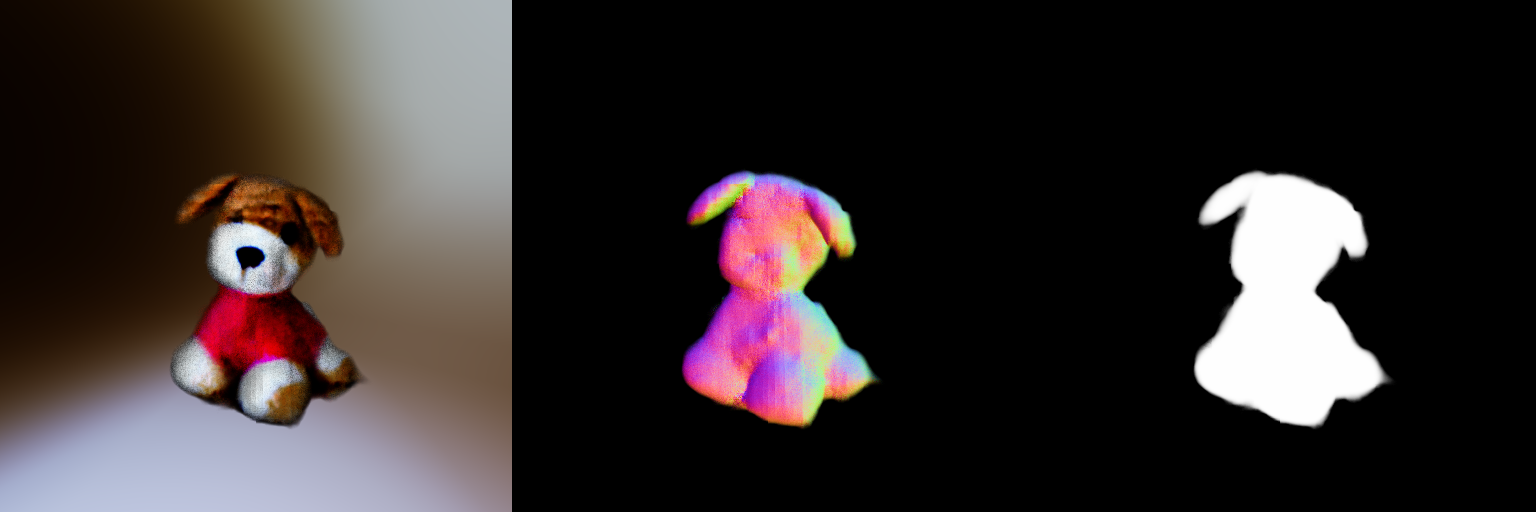
\includegraphics[width=\columnwidth]{report_task1_figures/obj_b.png}
  \caption{Object B plush puppy: lambertian, normal, and mask of 12{,}000-step SDS exported mesh, front view.}
  \label{fig:t1-object-b}
\end{figure}

In the front view of Fig.~\ref{fig:t1-object-b}, lambertian texture is complete, mask contour is clear, and the normal field is continuous and smooth in the head region---directly related to training view sampling bias: text defaults to front semantics and front elevation angles are sampled more frequently, so front SDS constraints accumulate more fully and front surface quality is best. But in the side view of Fig.~\ref{fig:t1-fusion}, obvious multi-face, multi-leg structural distortion appears. This is not an implementation bug but inherent SDS behavior: score estimates per view are independent; ``front looks like a dog'' and ``side looks like a dog'' can coexist as local optima; NeRF's continuous density field lacks hard topological constraints and cannot exclude redundant geometry, converging to a multi-faced body satisfying frequently sampled view semantics---the Janus problem.

\tabref{tab:t1-b-sds} shows SDS loss oscillates throughout with no monotonic convergence trend, so it should not be used as a convergence criterion. SDS gradients contain dual randomness: random camera sampling each step and random diffusion timestep $t$, causing optimization direction fluctuation and loss random walk rather than deterministic descent.

\begin{table}[H]
  \centering
  \caption{Object B SDS and regularization term losses}
  \label{tab:t1-b-sds}
  \footnotesize
  \adjustbox{max width=\columnwidth}{%
  \begin{tabular}{@{}rcccc@{}}
    \toprule
    step & loss\_sds & loss\_opaque & loss\_orient & loss\_sparsity \\
    \midrule
    0 & 7522 & 0.165 & 0.0168 & 0.258 \\
    2000 & 49.4 & 0.0876 & 0.0195 & 0.401 \\
    4000 & 2177 & 0.0712 & 0.0278 & 0.609 \\
    6000 & 4060 & 0.0477 & 0.0286 & 0.335 \\
    7999 & 157.3 & 0.0342 & 0.00665 & 0.336 \\
    11999 & 182.9 & 0.0413 & 0.0135 & 0.374 \\
    \bottomrule
  \end{tabular}}
  \tablenote{Note: Steps 0--7999 from first 8{,}000-step run; step 11999 from final 12{,}000-step run, from \texttt{object\_B/csv\_logs/version\_0/metrics.csv}.}
\end{table}

Among regularizers, opacity loss (\texttt{loss\_opaque}) drops from 0.165 to 0.0342, indicating dense object surfaces forming with complete foreground contours at most views; but sparsity loss (\texttt{loss\_sparsity}) stays high at 0.3--0.6 without sustained decrease. Sparsity regularization only penalizes globally excessive opacity and cannot distinguish ``single dense object'' from ``multiple overlapping semi-transparent structures''; Janus redundant geometry continuously consumes density budget, preventing further sparsity reduction.

Comparing 8000-step versus 12000-step metrics, extending training shows no essential change in SDS loss magnitude or oscillation; opacity and sparsity remain in the same range with only slight front-texture refinement and no side-view Janus improvement. This directly confirms the precision ceiling of pure text SDS: topological defects stem from problem underdetermination---without 3D observation constraints, infinitely many text-consistent local optima exist and stacking steps cannot break underdetermination boundaries; compute cannot replace observation. Total path time 3267\,s, with compute mainly from per-iteration diffusion U-Net backprop, further validating the mismatch between generative-path compute bottleneck and precision ceiling.

\subsection{Object C: Magic123 Single-View Reconstruction}

Object~C single-view generation sits between ``real observation anchoring'' and ``diffusion prior completion'': the input front photo provides deterministic pixel-level photometric constraint as a strong anchor; the coarse stage combines Zero123 3D view prior with Stable Diffusion semantic prior to extrapolate invisible regions; the fine stage converts implicit NeRF to explicit DMTet mesh for further geometry and texture refinement under fixed topology.

\begin{figure}[H]
  \centering
  \includegraphics[width=\columnwidth]{report_task1_figures/objectC_curve.png}
  \caption{Object C Magic123 coarse/fine training loss.}
  \label{fig:t1-curve-c}
\end{figure}

Fig.~\ref{fig:t1-curve-c} shows distinctly different optimization dynamics between coarse and fine stages, rooted in dual changes of geometric representation and supervision weight.

Coarse-stage \texttt{loss\_total} plunges from 1.014 at step 1 to 0.0366 within 500 steps (96.4\% drop), reaching 0.0262 at 1000 steps. Early rapid convergence comes from triple deterministic constraints: input RGB, foreground mask, and Zero123 view-consistency prior jointly provide clear optimization direction; the NeRF field quickly fits front geometry and contour, hence cliff-like loss drop. Step 2000 rebounds to 0.0388 as \texttt{loss\_rgb} rises from 0.00904 to 0.0161 and \texttt{loss\_mask} from 0.00632 to 0.0121---not instability but inevitable optimization shift: after front regions are fitted, focus moves to invisible side/back where diffusion SDS dominates underdetermined regions; its randomness perturbs the partially converged front implicit field, raising photometric and contour loss synchronously; as back geometry frames form, perturbation weakens and by 5000 steps converges to 0.00958 with \texttt{loss\_rgb} 0.00242 and \texttt{loss\_mask} 0.000305 in low oscillation.

Fine stage inherits coarse geometry with starting point only 0.0813; \texttt{loss\_rgb} drops to $4.6{\times}10^{-4}$ within 100 steps; monotonic descent to \texttt{loss\_total} 0.00475 at 5000 steps, late-stage (500--5000) stdev only 0.0028 in stable refinement plateau. Low-variance fast convergence stems from: (1) geometry compressed from infinite DoF NeRF to fixed-topology DMTet mesh, narrowing optimization space without large implicit-field fluctuations; (2) reduced SDS weight with input pixel photometric supervision dominating, gradients driven by deterministic reprojection error while diffusion prior is weak regularization, yielding smooth loss without large swings. Fine \texttt{loss\_rgb} reaches $1.24{\times}10^{-4}$ at 1000 steps then plateaus at $1.2{\sim}1.6{\times}10^{-4}$, roughly 15$\times$ below coarse end because explicit rasterization removes volume-rendering integration smoothing: NeRF integration blurs high-frequency detail imposing a pixel-error floor; DMTet mesh rasterization backprops precisely to vertices/textures enabling finer detail and lower photometric loss. \texttt{loss\_mask} declines from 0.0286 to 0.00385, numerically higher than coarse soft mask but corresponding to sharper hard boundaries. Together: coarse rapidly builds rough geometry amid diffusion noise; fine achieves low-variance convergence under deterministic photometric supervision with fixed DMTet topology.

\begin{figure}[H]
  \centering
  \begin{minipage}[t]{0.48\columnwidth}
    \centering
    \includegraphics[width=\linewidth]{report_task1_figures/obj_c_coarse.JPG}
    \captionof{figure}{Object C guitar Magic123 coarse stage: four-view lambertian / depth / normal / mask.}
    \label{fig:t1-object-c-coarse}
  \end{minipage}\hfill
  \begin{minipage}[t]{0.48\columnwidth}
    \centering
    \includegraphics[width=\linewidth]{report_task1_figures/obj_c_fine.JPG}
    \captionof{figure}{Object C guitar Magic123 fine stage: four-view renders sharper than coarse.}
    \label{fig:t1-object-c-fine}
  \end{minipage}
\end{figure}

In Fig.~\ref{fig:t1-object-c-coarse} coarse results, the most prominent phenomenon is back renders highly similar to front, with strings, sound hole, and pickguard on what should be a flat back---inconsistent with real guitar physics. Mechanism: input is only a single front image; invisible regions rely entirely on Zero123 and SD priors. Zero123 learns not strict physical 3D reconstruction but statistical ``pixel distribution after viewpoint rotation''; training data contains many symmetric objects inducing ``front-back similarity'' bias. Text prompt also emphasizes front features, guiding diffusion to generate front semantics on the back. Together the model ``copies'' front features to minimize SDS loss---the statistical optimum under single-view underdetermination with generative priors, not an implementation defect.

In the fine stage, geometry switches from NeRF implicit field to DMTet explicit mesh with reduced diffusion loss weight. \tabref{tab:t1-magic123} shows lambertian (RGB) loss dropping from coarse-end 0.00242 to fine-end $1.60{\times}10^{-4}$, with noticeably sharper four-view renders. Mechanism: explicit mesh compresses optimization from infinite continuous density to fixed vertices and texture parameters; input pixel photometric supervision dominates while diffusion prior becomes weak regularization, yielding more deterministic gradients and lower pixel error.

\begin{table}[H]
  \centering
  \caption{Object C Magic123 stage-wise losses}
  \label{tab:t1-magic123}
  \footnotesize
  \adjustbox{max width=\columnwidth}{%
  \begin{tabular}{@{}lccc@{}}
    \toprule
    Stage & loss\_total & loss\_lambertian & loss\_mask \\
    \midrule
    coarse @1 & 1.014 & 0.312 & 0.697 \\
    coarse @1000 & 0.0262 & 0.00904 & 0.00632 \\
    coarse @5000 & 0.00958 & 0.00242 & 0.000305 \\
    fine @1 & 0.0813 & 0.0394 & 0.0286 \\
    fine @1000 & 0.00914 & 0.000124 & 0.00772 \\
    fine @5000 & 0.00475 & 0.000160 & 0.00385 \\
    \bottomrule
  \end{tabular}}
  \tablenote{Note: Log field is \texttt{loss\_rgb}, listed as loss\_lambertian in table.}
\end{table}

Notably, mask loss rises from 0.000305 to 0.00385 in fine stage---not quality degradation but a numerical illusion from representation change: coarse NeRF mask from volume-rendered density is a soft probabilistic contour; loss against similarly soft GT is naturally small but visually blurry; fine mesh has sharp hard binary boundaries with mask supervision on edge pixels, so loss is higher but contours are clearer and more physically plausible.

After refinement, neck string structure remains overly smooth, lacking thin real string texture. Two constraints apply: single-view input provides no stereo parallax for sub-pixel string width; DMTet mesh resolution caps sub-millimeter thin structures---diffusion priors also smooth high-frequency thin structure to continuous texture, limiting accuracy by input information and representation capacity.

Full pipeline totals 6534\,s (coarse 3133\,s, fine 3362\,s, similar magnitude). Both stages share the same bottleneck: diffusion U-Net forward/backprop each step; NeRF volume rendering versus mesh rasterization is negligible relative to large diffusion inference, so switching to explicit mesh does not reduce total time by an order of magnitude, further validating diffusion backprop as the core generative-3D compute bottleneck.

\subsection{Background Scene, Fusion Preview, and Orbit Video}
\label{sec:t1-fusion-results}

Background uses Mip-NeRF 360 garden unbounded scene, training 2DGS 10{,}000 iter under public COLMAP poses with mesh resolution 1024 (\tabref{tab:t1-hparams}).

Fig.~\ref{fig:t1-curve-garden} and \tabref{tab:t1-2dgs-garden} show garden background training and validation. Curve morphology sharply contrasts with Object~A, essentially because geometric identifiability boundaries differ between unbounded large scenes and small-object reconstruction. Initial total loss 0.279 ($\sim$4.4$\times$ Object~A's 0.063), reflecting wide initial Gaussian distribution and large deviation from true surfaces in unbounded scenes.

(I) iter 1--2000: mean loss $\sim$0.135, dropping to 0.090 at 2000 iter, PSNR from 24.13\,dB, L1 0.0424. Rapid descent is driven entirely by near-field: stone table, pots have large parallax and strong multi-view constraints; Gaussians quickly align true surfaces contributing main loss drop; distant vegetation/sky have weak parallax with sparse misaligned Gaussians not yet effectively optimized, so PSNR starts much lower than small-object reconstruction.

(II) iter 2000--5000: loss continues to training minimum 0.0583 at 5000 iter; PSNR 25.06\,dB, L1 0.0363 at 4000 iter. Optimization spreads from near to mid field; densification supplements mid/far Gaussians filling geometric gaps; normal regularization not yet active, optimization purely photometric, so training loss decreases monotonically and PSNR rises steadily.

(III) iter 5000--6000: PSNR jumps to peak 26.63\,dB (+1.57\,dB) while loss rebounds to 0.0667---early ``validation improves, training loss rises.'' Core cause is large-scale densification transients: mid/far Gaussian split/completion concentrates, new Gaussians temporarily raise training loss but fill geometric blind spots improving large-scene render completeness, hence validation PSNR step gain. Unbounded densification covers wider range with more new Gaussians than small objects, so loss rebound and PSNR jump are more pronounced.

(IV) iter $\geq$7000 with normal regularization: total loss jumps to 0.0789 and stabilizes at 0.0834 while PSNR plateaus 26.52--26.68\,dB (0.16\,dB fluctuation), L1 stable 0.0305--0.0312. Plateau reflects unbounded identifiability bottleneck: far regions have negligible parallax, multi-view pixel differences near sensor noise, photometric gradients ineffective, far Gaussians cannot improve further; far pixels exceed half the image locking overall PSNR ceiling. Normal-regularization loss increment mainly regularizes vast far Gaussians contributing little PSNR weight, so training loss rises 43\% while validation barely changes---regularization cost concentrates in low-weight regions without harming core-view quality.

\enlargethispage{2\baselineskip}
\begin{table}[H]
  \centering
  \caption{Garden background 2DGS training and validation metrics}
  \label{tab:t1-2dgs-garden}
  \footnotesize
  \setlength{\tabcolsep}{4pt}
  \begin{tabular}{@{}rcccc@{}}
    \toprule
    iter & val PSNR (dB) & val L1 & train loss & normal \\
    \midrule
    1 & --- & --- & 0.279 & 0 \\
    2000 & 24.13 & 0.0424 & 0.0900 & 0 \\
    4000 & 25.06 & 0.0363 & 0.0773 & 0 \\
    5000 & --- & --- & 0.0583 & 0 \\
    6000 & 26.63 & 0.0305 & 0.0667 & 0 \\
    7000 & --- & --- & 0.0789 & 0 \\
    8000 & 26.52 & 0.0312 & 0.0713 & 0.0181 \\
    10000 & 26.68 & 0.0305 & 0.0834 & 0.0155 \\
    \bottomrule
  \end{tabular}
  \tablenote{Note: val columns are hold-out evaluation every 2000 iter; normal regularization from iter $\geq$7000.}
\end{table}
\begin{figure}[H]
  \centering
  \includegraphics[width=\columnwidth]{report_task1_figures/garden_curve.png}
  \caption{Garden background 2DGS training loss and validation PSNR.}
  \label{fig:t1-curve-garden}
\end{figure}

\begin{figure}[H]
  \centering
  \includegraphics[width=\columnwidth]{report_task1_figures/garden.jpg}
  \caption{Garden background 2DGS four-view novel renders.}
  \label{fig:t1-background}
\end{figure}

Fig.~\ref{fig:t1-background} four novel views match PSNR 26.68\,dB: near stone table, pots, and plants with sharp edges and discernible texture; distant vegetation and sky slightly smooth due to weak parallax, matching plateau metrics. This ``sharp near, smooth far'' layering is inherent to unbounded multi-view reconstruction, not algorithm failure: near-field high fidelity validates 2DGS effectiveness; far smoothness reflects parallax insufficiency physical limit that more training cannot break. Garden full pipeline 2841\,s (2DGS 1984\,s + mesh export 857\,s).

Four heterogeneous 3D assets export uniformly as triangle meshes then import into Blender for fusion---a compromise balancing compatibility and precision: 2DGS surfels convert to mesh via Poisson reconstruction; generative implicit fields export via isosurface extraction; both unify at mesh level solving representation heterogeneity, Fig.~\ref{fig:t1-fusion}.

\begin{figure}[H]
  \centering
  \includegraphics[width=\columnwidth]{report_task1_figures/all_object.JPG}
  \caption{Multi-object and garden background fusion: three-view orbit static frames.}
  \label{fig:t1-fusion}
\end{figure}

Fig.~\ref{fig:t1-fusion} three-view comparison: sneaker and guitar geometry credible with natural table contact; plush puppy acceptable frontally but side view shows multi-face multi-leg Janus (echoing high-PSNR path in \S\ref{sec:t1-object-a-results} and SDS analysis above). This intuitively demonstrates multi-source ``bottleneck effect'': final fusion visual quality ceiling is determined by the weakest-supervision, lowest-precision asset. Blender material/lighting matching only optimizes appearance consistency; it cannot fix SDS Janus topology or fill in single-view missing back detail; post-compositing can mask some flaws but cannot break native generation precision ceiling.

\begin{figure}[H]
  \centering
  \adjustbox{trim=0 0 0 350pt,clip,width=\columnwidth}{%
    \includegraphics{report_task1_figures/wandering_frame.jpg}%
  }
  \caption{Orbit wandering video representative frame, frame 60.}
  \label{fig:t1-wandering}
\end{figure}

Fig.~\ref{fig:t1-wandering} is frame 60 of \texttt{wandering.mov}: camera orbits fused scene with coherent lighting; parallax natural without penetration/floating, showing mesh export and spatial alignment precision; puppy side still shows Janus artifacts, guitar neck slightly softer than single-object render from multi-asset color temperature and material differences---unified light baking could further optimize without affecting core fusion conclusions.

On compute scale sensitivity: 2DGS training time scales roughly with scene size and Gaussian count; garden Gaussians far exceed single objects so training time is $\sim$4$\times$ Object~A, showing differentiable rasterization efficiency grows gently with scale; generative path time is dominated by diffusion call count, nearly independent of object size, so simple ornaments and complex instruments share similar generation time. Overall compute distribution again confirms: real multi-view observation is the core source of geometric precision and the most compute-efficient path; generative schemes offer zero-shot flexibility but far lower geometric precision per unit compute with hard underdetermination bottlenecks.

\section{Discussion}
\label{sec:t1-discuss}
%==============================================================================

\subsection{Comparison of Three Reconstruction Paradigms}

\begin{table*}[!t]
  \centering
  \caption{Three input paradigms compared: geometric accuracy, texture detail, and compute time}
  \label{tab:t1-three-way}
  \footnotesize
  \setlength{\tabcolsep}{4pt}
  \begin{tabular}{@{}>{\raggedright\arraybackslash}p{0.10\textwidth}>{\raggedright\arraybackslash}p{0.14\textwidth}>{\raggedright\arraybackslash}p{0.26\textwidth}>{\raggedright\arraybackslash}p{0.24\textwidth}>{\raggedright\arraybackslash}p{0.14\textwidth}r@{}}
    \toprule
    Paradigm (object) & Supervision & Geometric accuracy & Texture detail & Key metric & Time (s) \\
    \midrule
    Multi-view 2DGS\newline (sneaker A) &
    36 self-captured orbit photos with COLMAP; photometric reprojection + $\lambda_{\mathrm{mask}}{=}0.1$ + normal reg. &
    Orbit-consistent topology, no Janus. Hold-out PSNR 36.12\,dB. Fig.~\ref{fig:t1-object-a} renders align with GT in silhouette, sole texture, side thickness &
    Fabric direction, brand logo, lace holes stable across views; shading matches capture, no floaters or background leak &
    PSNR 36.12\,dB\newline L1 0.00391 &
    542 \\
    \addlinespace[2pt]
    Text SDS\newline (puppy B) &
    No capture; positive prompt for round head, short snout, drooping ears, solid torso; negative prompt suppresses multi-face/legs; SD v1.5 score distillation, zero 3D GT &
    Front elevation lambertian/normal/mask dense and continuous (Fig.~\ref{fig:t1-object-b}), but fusion side view shows multi-face multi-leg Janus (Fig.~\ref{fig:t1-fusion}). $\mathcal{L}_{\mathrm{opaque}}$ drop only indicates renderable surface, not simply-connected topology; 12{,}000 steps, side distortion persists &
    Front warm-brown fur, red vest, white muzzle clear at training views; orbit back/side entirely diffusion-hallucinated, semantically plausible but not physically consistent &
    $\mathcal{L}_{\mathrm{SDS}}$ oscillates; opaque $\to$0.034, sparsity still 0.3--0.6; no hold-out PSNR &
    3267 \\
    \addlinespace[2pt]
    Single-image Magic123\newline (guitar C) &
    Single front photo RGB anchor; coarse joint Zero123 view + SD semantic prior; fine DMTet with strengthened input-view supervision &
    Input-view body contour and sound-hole position accurate. Coarse back copies front: strings and sound hole on flat back (Fig.~\ref{fig:t1-object-c-coarse}), Zero123 symmetry bias. Fine four-view edges sharpened (Fig.~\ref{fig:t1-object-c-fine}), neck strings still overly smooth &
    Front spruce top, tortoiseshell pickguard, metal tuners faithful at input view; coarse side dirty/blurry, fine lambertian $\sim$15$\times$ lower than coarse, still lacks string-level high-frequency detail &
    coarse RGB 0.00242\newline fine RGB $1.6{\times}10^{-4}$; no multi-view GT PSNR &
    6534 \\
    \bottomrule
  \end{tabular}
  \tablenote{Note: Time is per-object core path wall clock (A: COLMAP+2DGS+export; B: SDS 12{,}000 steps; C: preprocess+coarse+fine). B and C diffusion backprop total 9762\,s, 74.0\% of four paths.}
\end{table*}

The core divide among three paradigms lies in constraint strength on the 3D solution space, corresponding to overdetermined, semi-constrained, and underdetermined problem forms; differences in geometric precision, texture quality, and compute cost are endogenously determined by constraint properties, not model structure or training steps (detailed comparison in \tabref{tab:t1-three-way}).

From geometric identifiability: multi-view 2DGS transforms 3D reconstruction from ill-posed inverse problem to uniquely constrained optimization via real multi-view observations; geometric fidelity ceiling is directly determined by observation density. Pure text SDS has no 3D ground truth; solution space has infinitely many semantics-consistent local optima; Janus and other topological defects are inevitable underdetermined outcomes that cannot be broken by simply extending training. Single-image generation is intermediate: input image anchors front solution space while generative priors fill invisible regions, so front precision nears real reconstruction but underdetermined regions show symmetry errors from prior statistical bias.

From precision--compute marginal returns: multi-view path compute scales roughly linearly with scene size, stably converting unit compute to geometric precision; generative paths show strong diminishing returns---early rapid semantic contour formation, then SDS gradient randomness prevents sustained geometric gains, with most compute oscillating among local optima. Experimentally diffusion training is 74\% of total time yet contributes far less geometric precision gain than multi-view reconstruction at only 4.1\% share, illustrating order-of-magnitude cost-effectiveness difference.

From applicable scenario boundaries: no paradigm is absolutely superior; each maps to different needs. Multi-view 2DGS suits real-scene reconstruction with capture conditions and high topology/texture consistency requirements; pure text SDS suits zero-observation creative concept generation and rapid prototyping with low geometric correctness demands; single-image generation suits single-reference rapid 3D completion balancing input-view precision and generative flexibility.

\subsection{Limitations and Future Work}

Quantitatively, generative paths lack 3D ground truth and cannot share unified geometric error metrics with reconstruction paths; current evaluation is qualitative plus component metrics with limited cross-path quantitative comparison.

Fusion uses triangle mesh as unified intermediary for heterogeneous asset stitching---compatible but loses 2DGS native view-dependent effects (specular, translucency); fused scenes are limited to Lambertian material assumption.

Generation defects: text Janus and single-image symmetry bias are both prior biases in underdetermined regions; no additional constraints currently correct them.

Compute efficiency: diffusion backprop is 74\% of total time with substantial redundant computation.

Future work: (1) explore direct Gaussian-level scene fusion without mesh export preserving 2DGS native rendering; (2) introduce monocular depth or sparse views as weak supervision correcting symmetry bias and suppressing Janus; (3) optimize diffusion paths via viewpoint score caching and distilled small-step models reducing per-iteration cost; (4) build unified multi-paradigm quality benchmarks enabling quantitative cross-path comparison.

%==============================================================================
\section{Conclusion}
\label{sec:t1-conclusion}
%==============================================================================

We fully implement multi-view 2DGS real reconstruction, text-driven SDS generation, and single-view Magic123 generation, completing multi-source asset fusion in real outdoor scenes via unified triangle mesh representation with orbit video output. Comparing three paradigms across supervision mechanism, optimization dynamics, and compute efficiency, we conclude: 3D asset geometric identifiability and quality ceiling are fundamentally determined by supervision source and dimension, not training steps or model capacity.

From underlying geometric precision constraints, three paradigms correspond to overdetermined, semi-constrained, and underdetermined forms with endogenous precision ceilings. Multi-view 2DGS with 36 orbit observations and precise poses transforms reconstruction into uniquely constrained optimization; surfel direct gradient conduction reaches 36.12\,dB novel-view rendering in 542\,s core time---optimal geometric fidelity and efficiency. Pure text SDS is fully underdetermined with only 2D diffusion semantic priors; infinitely many text-consistent local optima exist; Janus multi-face topology is inherent; even 12000 steps cannot eliminate it, validating compute stacking cannot break identifiability ceiling from missing observations. Single-view Magic123 is semi-constrained hybrid: single photo anchors front with strong pixel supervision; invisible regions filled by Zero123 view prior balancing input cost and quality; but symmetry inductive bias causes back structure-copy errors and two-stage diffusion backprop yields 6534\,s highest total time.

From compute cost-effectiveness: diffusion backprop is the core bottleneck of generative paths; B and C diffusion training totals 74.0\% of core time. Multi-view real reconstruction shows roughly linear compute-to-precision returns with stable marginal benefit; generative paths show strong diminishing returns---early semantic contour gains, then SDS randomness traps most compute in local-optima oscillation without sustained geometric gains. Where real observations can be added, multi-view capture cost-effectiveness far exceeds extending generative iterations.

Fusion results confirm 3D generation ``bottleneck effect'': heterogeneous fusion visual quality ceiling is determined by weakest-supervision path. Unified triangle mesh only solves format compatibility; later lighting/material matching optimizes appearance consistency but cannot remedy topology defects and geometric errors from insufficient supervision during generation; post-compositing cannot break native generation precision ceiling. This provides clear technical selection guidance: prefer multi-view real reconstruction when topology consistency and capture are available; use pure text generation for zero-observation creative prototypes; use single-image generation as balanced compromise when only one reference exists needing front precision and efficiency.

\part{LeRobot ACT Cross-Environment Generalization}

%==============================================================================
\section{Introduction}
\label{sec:t2-intro}
%==============================================================================

\subsection{Background and Motivation}

Vision-motor policies replicate expert trajectories on fixed benches but degrade sharply under deployment environment changes (texture, layout, lighting), attributed to compounding error and distribution shift\cite{ross2011dagger,codevilla2019exploring}. Zero-shot cross-environment generalization requires extracting task-relevant invariances rather than memorizing environment-specific spurious features.

The CALVIN benchmark\cite{mees2022calvin} maintains task semantics and robot embodiment across four visual scenes (A--D), decoupling task difficulty from visual domain change. We compare single-environment training (B) versus multi-environment mixed training (ABC\_fair) on official LeRobot ACT\cite{zhao2023learning,cadene2024lerobot}, with zero-shot evaluation on unseen environment D to isolate training data breadth effects and examine Action Chunking error evolution under visual shift.

\subsection{Related Work}

Behavior cloning (BC) treats expert policy as supervised learning; Ross et al.\cite{ross2011dagger} show per-frame BC error accumulates over time. ACT\cite{zhao2023learning} uses Transformer to predict action chunks with conditional VAE for multimodality, outperforming traditional BC on fine manipulation. For visual change, domain randomization\cite{tobin2017domain} and multi-environment joint training expand training observation distribution; De Haan et al.\cite{dehaan2019causal} note policies may rely on non-causal background factors and fail on extrapolation. CALVIN\cite{mees2022calvin} provides four switchable scenes; LeRobot\cite{cadene2024lerobot,lerobot2025datasetv3} unifies data to LeRobotDataset v3.0. We use \texttt{lerobot-train} official pipeline, widening training visual distribution via multi-environment data without algorithm changes.

\subsection{Research Objectives and Contributions}

We construct Exp-B / Exp-ABC\_fair controls (ResNet-18 ACT, $H{=}100$, $k{=}10$, AdamW, batch 16, seed 42, 80k steps), reporting L1, quantiles, per-dimension decomposition, chunk step-wise $\bar{L}_k$, and proxy success rate in normalized action space. Empirically: single-env B has lower in-dist L1 (0.310 vs.\ 0.390) but larger generalization gap on D (0.212 vs.\ 0.073); mixed training reduces max chunk step gap from 0.297 to 0.103 while $\rho\approx1.5$ nearly unchanged. CALVIN original benchmark emphasizes language-conditioned long-horizon task chains\cite{mees2022calvin}; our ACT uses only RGB and proprioception (\S\ref{sec:dataset-policy}), no language, focusing on pure visuomotor cross-environment generalization.

%==============================================================================
\section{Dataset and Evaluation Protocol}
%==============================================================================

\subsection{CALVIN-Style Data and Scene Splits}

CALVIN\cite{mees2022calvin} uses Franka arm in PyBullet for grasp/place atomic skills; Multi-Environment protocol switches among four visual scenes A--D. Our data is converted to LeRobotDataset v3.0\cite{lerobot2025datasetv3} at \texttt{task2/data/calvin\_env\_\{A,B,C,ABC,D\}}. Five split sizes in \apptabref{apptab:data-full}: single-env A/B/C each $\sim$4467--4468 episodes, 268k frames; mixed ABC 13403 episodes, 804{,}370 frames; held-out D 4467 episodes, 267{,}373 frames.

Exp-B reads only \texttt{calvin\_env\_B}; ABC\_fair reads \texttt{calvin\_env\_ABC} (A+B+C concatenated). D is never seen during training, used only for zero-shot offline evaluation. Task semantics and action space are consistent across environments; differences are mainly background, table material, and layout in third-person view.

\subsection{LeRobot v3.0 Data Format and Storage}

LeRobotDataset v3.0 stores \texttt{observation.state}, \texttt{action}, etc.\ in Parquet; third-person and wrist RGB in AV1 MP4 ($256{\times}256$, 30\,fps); metadata in \texttt{meta/info.json}, \texttt{meta/stats.json}, \texttt{meta/episodes/}. Local script \texttt{verify\_dataset.py} checks split integrity.

\subsection{Observations, Actions, and Policy Interface}
\label{sec:dataset-policy}

\tabref{tab:features} summarizes ACT inputs/outputs (from checkpoint \texttt{config.json} and \texttt{meta/info.json}). Despite \texttt{annotation.human.action.task\_description} (language task ID) in data, the policy receives no language, only vision and proprioception, isolating visual distribution shift effects on action regression.

\begin{table}[H]
  \centering
  \caption{Policy I/O and dataset features used in this work}
  \label{tab:features}
  \footnotesize
  \adjustbox{max width=\columnwidth}{%
  \begin{tabular}{@{}llll@{}}
    \toprule
    Field & Shape / type & Modality & Usage \\
    \midrule
    \texttt{observation.images.image} & $256{\times}256{\times}3$ video & VISUAL & ACT input \\
    \texttt{observation.images.wrist\_image} & $256{\times}256{\times}3$ video & VISUAL & ACT input \\
    \texttt{observation.state} & $\mathbb{R}^{15}$ & STATE & ACT input \\
    \texttt{action} & $\mathbb{R}^{7}$ & ACTION & ACT output / loss \\
    \texttt{task\_index} / language ann. & int64 & --- & Not used by ACT \\
    \bottomrule
  \end{tabular}}
\end{table}

7-D action follows CALVIN/LeRobot convention: $(\mathrm{pos}_x,\mathrm{pos}_y,\mathrm{pos}_z,\mathrm{rot}_x,\mathrm{rot}_y,\mathrm{rot}_z,\mathrm{gripper})$, rotation as Euler angles. Preprocessor applies MEAN\_STD normalization to VISUAL/STATE/ACTION (statistics from training split, frozen in checkpoint); all L1 metrics below are in normalized action space.

\subsection{Notation}

\apptabref{apptab:notation} summarizes main notation. Unless noted, all action errors are computed in preprocessor-normalized 7-D action space.

\subsection{Training-Time Data Processing}

Training script \texttt{scripts/train.sh} calls LeRobot data pipeline via \texttt{lerobot-train}. Data loads locally offline (\texttt{HF\_HUB\_OFFLINE=1}, \texttt{repo\_id=local/calvin\_env\_*}); CUDA video decode uses \texttt{torchcodec}, else \texttt{pyav} fallback. Image augmentation disabled (\texttt{image\_transforms.enable=false}); ACT samples $H{=}100$ continuous trajectory windows with \texttt{action\_is\_pad} masking episode tail padding. Reproducibility via \texttt{SEED=42} and \texttt{cudnn\_deterministic=true}; server mode uses full episodes, smoke mode only \texttt{episodes=[0,1,2]}, 20 steps. Settings summarized in \tabref{tab:data-pipeline}.

\begin{table}[H]
  \centering
  \caption{Training-time data pipeline settings}
  \label{tab:data-pipeline}
  \footnotesize
  \adjustbox{max width=\columnwidth}{%
  \begin{tabular}{@{}>{\raggedright\arraybackslash}p{0.28\columnwidth}>{\raggedright\arraybackslash}p{0.68\columnwidth}@{}}
    \toprule
    Item & Setting \\
    \midrule
    Data loading & Local offline, \texttt{root=task2/data/calvin\_env\_*} \\
    Video backend & \texttt{torchcodec} (CUDA) / \texttt{pyav} (fallback) \\
    Augmentation & Disabled \\
    Trajectory window & $H{=}100$, pad mask via \texttt{action\_is\_pad} \\
    Reproducibility & \texttt{SEED=42}, \texttt{cudnn\_deterministic=true} \\
    \bottomrule
  \end{tabular}}
\end{table}

\subsection{Evaluation Metric Definitions}

All metrics computed by \texttt{scripts/eval\_zeroshot.py} under \texttt{torch.inference\_mode()}: per frame call \texttt{policy.predict\_action\_chunk}, compute element-wise L1 against GT chunk, mask invalid steps with \texttt{action\_is\_pad}.

\subsubsection{Frame-Level L1 Error}

For frame $i$, average over valid chunk steps and 7 action dimensions to scalar $\ell_i$; dataset-level error
\begin{equation}
  \mathcal{L}_{\mathrm{L1}} = \frac{1}{N}\sum_{i=1}^{N} \ell_i,
  \label{eq:l1}
\end{equation}
corresponding to JSON field \texttt{action\_l1\_loss}. Also report median, $p_{10}$, $p_{90}$, $p_{95}$ for typical and tail frames.

\subsubsection{Generalization Gap}

\begin{equation}
  \Delta_{\mathrm{abs}} = \mathcal{L}_{\mathrm{L1}}^{\mathrm{D}} - \mathcal{L}_{\mathrm{L1}}^{\mathrm{in\text{-}dist}},\qquad
  \Delta_{\mathrm{rel}} = \mathcal{L}_{\mathrm{L1}}^{\mathrm{D}} \big/ \mathcal{L}_{\mathrm{L1}}^{\mathrm{in\text{-}dist}}.
  \label{eq:gap}
\end{equation}
Merged from in-dist and zero-shot JSON by \texttt{summarize\_eval.py}.

\subsubsection{Chunk Step-Wise Error and Horizon Degradation}

Let $\bar{L}_k$ be mean L1 at chunk step $k$ over all valid frames (7-D action averaged first), corresponding to \texttt{chunk\_step\_l1[k]}. Define
\begin{equation}
  \rho = \bar{L}_{K-1} / \bar{L}_0,\quad K=65\;(k=0,\ldots,64),
  \label{eq:deg}
\end{equation}
i.e., \texttt{chunk\_horizon\_degradation}. Also report \texttt{max\_chunk\_step\_gap}$=\max_k(\bar{L}_k^{\mathrm{D}}-\bar{L}_k^{\mathrm{in}})$ and its step index.

\subsubsection{Action Dimension Decomposition and Proxy Success Rate}

Per-dimension L1 accumulated independently as \texttt{action\_dim\_l1}. For thresholds $\tau\in\{0.05,0.1,0.5,1.0\}$,
\begin{equation}
  \mathrm{SR}_{\tau} = \frac{1}{N}\bigl|\{i : \ell_i < \tau\}\bigr|.
  \label{eq:sr}
\end{equation}
CALVIN official Success Rate is long-horizon language task chain completion in simulation\cite{mees2022calvin}; Eq.~(\ref{eq:sr}) is single-frame action accuracy proxy, not directly comparable to original task-level metrics.

\subsection{Offline Evaluation and Report Generation}

Full evaluation orchestrated by \texttt{eval\_report.sh}: in-distribution on respective training environments (B$\to$B, ABC\_fair$\to$ABC), then zero-shot on \texttt{calvin\_env\_D} with same checkpoint; \texttt{summarize\_eval.py} merges JSON, computes Eq.~(\ref{eq:gap}) and chunk step gaps; \texttt{plot\_eval\_metrics.py} and \texttt{eval\_compare.sh} generate chunk curves and gap bar charts. Server eval defaults \texttt{batch\_size=16}, \texttt{num\_workers=8}, \texttt{seed=42}, full frames; all table values from checkpoint \texttt{080000}.

%==============================================================================
\section{Method: LeRobot ACT Algorithm}
%==============================================================================

\subsection{ACT Core Principle and Comparison to Per-Frame BC}

ACT predicts an action sequence of length $H$, shortening effective horizon by $\sim H$ to mitigate compounding error\cite{ross2011dagger,zhao2023learning}. Given observation $o_t$ and state $s_t$, the policy learns
\begin{equation}
  p_\theta(\mathbf{a}_{t:t+H-1} \mid o_t, s_t, z),
  \label{eq:act}
\end{equation}
where $z$ is CVAE latent variable. Training objective
\begin{equation}
  \mathcal{L} = \underbrace{\| a - \hat{a} \|_1}_{\mathcal{L}_{\mathrm{L1}}}
  + \lambda_{\mathrm{kl}}\,
  \underbrace{\mathcal{D}_{\mathrm{KL}}\bigl(q_\phi(z|o,a)\,\|\,p(z)\bigr)}_{\text{prior regularization}},
  \label{eq:loss}
\end{equation}
$\lambda_{\mathrm{kl}}{=}10$. At inference, predict full chunk, execute first $k$ steps then replan; we use $H{=}100$, $k{=}10$.

\subsection{Network Architecture Details}

We use LeRobot 0.5.1 official ACT implementation; hyperparameters frozen in checkpoint \texttt{config.json} as in \tabref{tab:arch}, with no custom modifications.

\begin{table}[H]
  \centering
  \caption{ACT network architecture (from \texttt{config.json})}
  \label{tab:arch}
  \footnotesize
  \adjustbox{max width=\columnwidth}{%
  \begin{tabular}{@{}>{\raggedright\arraybackslash}p{0.34\columnwidth}>{\raggedright\arraybackslash}p{0.62\columnwidth}@{}}
    \toprule
    Module & Configuration \\
    \midrule
    Observation steps $n_{\mathrm{obs}}$ & 1 (single-frame conditioning) \\
    Vision backbone & ResNet-18, ImageNet-1K pretrained \\
    Backbone output & Per-camera feature maps $\to$ flattened tokens \\
    State encoder & Linear projection of $\mathbb{R}^{15}$ \\
    Transformer encoder & 4 layers, 8 heads, $d_{\mathrm{model}}{=}512$, FFN $=3200$ \\
    Transformer decoder & 1 layer, cross-attention to encoder tokens \\
    VAE encoder & 4 layers, latent dim $d_z{=}32$ \\
    Action head & 7-dim output per decoder step \\
    Dropout & 0.1 \\
    Activation (FFN) & ReLU \\
    Normalization & MEAN\_STD on VISUAL / STATE / ACTION \\
    \bottomrule
  \end{tabular}}
\end{table}

\subsubsection{Visual Encoding and Multi-Camera Fusion}

Two RGB streams pass through ResNet-18; linearly projected proprioception $s_t\in\mathbb{R}^{15}$ forms Transformer encoder input. ResNet uses ImageNet pretrained weights; backbone LR equals policy head ($10^{-5}$).

\subsubsection{Transformer Encoder-Decoder and Action Sequence Generation}

Encoder outputs context $\mathbf{c}_t$; decoder uses action position embeddings as queries, generating $H$ 7-D action vectors stepwise. LeRobot sets \texttt{temporal\_ensemble\_coeff=null}; no temporal ensembling at inference.

\subsection{Training and Inference Pipeline}

Training via \texttt{lerobot-train}, sampling continuous $H$-step trajectory windows; \texttt{action\_is\_pad} masks padded episode tails. Optimizer AdamW ($10^{-5}$, weight decay $10^{-4}$), gradient clip 10.0, checkpoint every 10{,}000 steps; results from 80{,}000 steps.

At inference, each frame calls \texttt{policy.predict\_action\_chunk}, outputting $\hat{\mathbf{a}}_{t:t+H-1}$; environment executes first $k{=}10$ steps. CALVIN original benchmark uses long-horizon task-chain success in simulation\cite{mees2022calvin}; we use frame-level offline L1 as reproducible proxy (\S\ref{sec:metrics-offline}) and analyze chunk step-wise errors.

%==============================================================================
\section{Experimental Setup}
%==============================================================================

\subsection{Experimental Design Overview}

Single-factor controlled design: sole independent variable is training data split (B vs.\ ABC); dependent variables are in-distribution/zero-shot action L1 and derived metrics. Two experiments Exp-B and Exp-ABC\_fair, summarized in \tabref{tab:exp-design}.

\begin{table}[H]
  \centering
  \caption{Controlled experimental conditions}
  \label{tab:exp-design}
  \footnotesize
  \adjustbox{max width=\columnwidth}{%
  \begin{tabular}{@{}lllll@{}}
    \toprule
    ID & Train data & Output dir & In-dist eval & Zero-shot eval \\
    \midrule
    Exp-B & \texttt{calvin\_env\_B} & \texttt{train\_b} & env B & env D \\
    Exp-ABC\_fair & \texttt{calvin\_env\_ABC} & \texttt{train\_abc\_fair} & env ABC & env D \\
    \bottomrule
  \end{tabular}}
\end{table}

Except differences in \tabref{tab:exp-design}, network, optimizer, seed, training steps, batch size, augmentation, video backend, and evaluation protocol are identical. Environment D never participates in gradient updates.

\subsection{Hardware and Software Environment}

All formal experiments on Alibaba Cloud GPU server, Conda env \texttt{task2} (or \texttt{venv}, \S\ref{sec:repro}). Software versions in \tabref{tab:software-env}; training throughput $\sim$11.3 step/s, $\sim$2 hours wall clock per experiment.

\begin{table}[H]
  \centering
  \caption{Hardware and software environment}
  \label{tab:software-env}
  \footnotesize
  \adjustbox{max width=\columnwidth}{%
  \begin{tabular}{@{}>{\raggedright\arraybackslash}p{0.3\columnwidth}>{\raggedright\arraybackslash}p{0.66\columnwidth}@{}}
    \toprule
    Component & Version / setting \\
    \midrule
    Compute & NVIDIA GPU, \texttt{device=cuda} \\
    Python & 3.12 \\
    PyTorch / torchvision & 2.10.0 / 0.25.0 (CUDA 12.1) \\
    LeRobot & 0.5.1, entry \texttt{lerobot-train} \\
    Env manager & Conda \texttt{task2} (\texttt{environment.yml}) \\
    Video decode & \texttt{torchcodec} (CUDA) / \texttt{pyav} (CPU) \\
    Logging & WandB 0.24.x, offline, project \texttt{cv\_hw3\_task2} \\
    Reproducibility & \texttt{SEED=42}, \texttt{CUDNN\_DETERMINISTIC=true} \\
    \bottomrule
  \end{tabular}}
\end{table}

\subsection{Training Hyperparameters and Controlled Variables}

\tabref{tab:hparams-train} lists full \texttt{train\_config.json}. Only \texttt{dataset.root}, \texttt{output\_dir}, \texttt{job\_name} differ; \tabref{tab:hparams} gives 80{,}000-step checkpoint IDs and epoch coverage.

\begin{table}[H]
  \centering
  \caption{Training configuration (\texttt{train\_config.json})}
  \label{tab:hparams-train}
  \footnotesize
  \adjustbox{max width=\columnwidth}{%
  \begin{tabular}{@{}>{\raggedright\arraybackslash}p{0.42\columnwidth}>{\raggedright\arraybackslash}p{0.54\columnwidth}@{}}
    \toprule
    Parameter & Value \\
    \midrule
    Policy type & ACT \\
    chunk\_size $H$ / n\_action\_steps $k$ & 100 / 10 \\
    batch\_size / num\_workers & 16 / 8 \\
    optimizer & AdamW ($\mathrm{lr}{=}10^{-5}$, wd${=}10^{-4}$, clip${=}10$) \\
    scheduler & None \\
    total training steps & 80{,}000 \\
    save\_freq / log\_freq & 10{,}000 / 100 \\
    eval\_freq & 0 (no online eval during training) \\
    seed / cudnn\_deterministic & 42 / true \\
    use\_amp & false \\
    kl\_weight $\lambda_{\mathrm{kl}}$ & 10 \\
    image\_transforms & disabled \\
    tolerance\_s & 0.02 \\
    video\_backend (CUDA) & torchcodec \\
    \bottomrule
  \end{tabular}}
\end{table}

\begin{table}[H]
  \centering
  \caption{Experiment identifiers at step 80{,}000}
  \label{tab:hparams}
  \footnotesize
  \adjustbox{max width=\columnwidth}{%
  \begin{tabular}{@{}llll@{}}
    \toprule
    Exp & WandB job / run & Final train L1 & Epoch coverage \\
    \midrule
    Exp-B & \texttt{act\_calvin\_b} / fp2i5ixm & 0.09481\textsuperscript{a} & $\sim$4.77 \\
    Exp-ABC\_fair & \texttt{act\_calvin\_abc\_fair} / c017f1db & 0.10770\textsuperscript{a} & $\sim$1.59 \\
    \bottomrule
  \end{tabular}}
  \tablenote{\textsuperscript{a}\texttt{task2/l1\_loss.csv} \texttt{train/l1\_loss} at step 80{,}000.}
\end{table}

\subsection{Optimization Steps and Epoch Coverage}

Controls align on gradient steps (80{,}000) not epochs. ABC mixed set (804{,}370 frames) is $\sim$3$\times$ B (268{,}201), so Exp-B covers $\sim$4.77 epochs vs.\ Exp-ABC\_fair $\sim$1.59 (\texttt{epch} in training log). ABC\_fair higher in-dist L1 (0.390 vs.\ 0.310) partly reflects data difficulty and insufficient epoch coverage. All evaluation uses \texttt{checkpoints/080000}.

\subsection{Offline Evaluation Configuration}
\label{sec:metrics-offline}

Offline eval uses outputs/train\_\{b,abc\_fair\}/check\\-points/080000; in-distribution on respective training env, zero-shot on D; \texttt{batch\_size=16}, \texttt{num\_workers=8}, \texttt{SEED=42}, full frames (B: 268{,}201; ABC: 804{,}370; D: 267{,}373), proxy SR thresholds $\tau\in\{0.05,0.1,0.5,1.0\}$, outputs \texttt{eval\_*.json}, \texttt{report\_*.json}, and figures. No online validation during training (\texttt{eval\_freq=0}); all generalization metrics computed post-training.

%==============================================================================
\section{Experimental Results and Analysis}
%==============================================================================

\subsection{Training Convergence Comparison}

\begin{figure*}[!t]
  \centering
  \begin{minipage}[t]{0.24\textwidth}
    \centering
    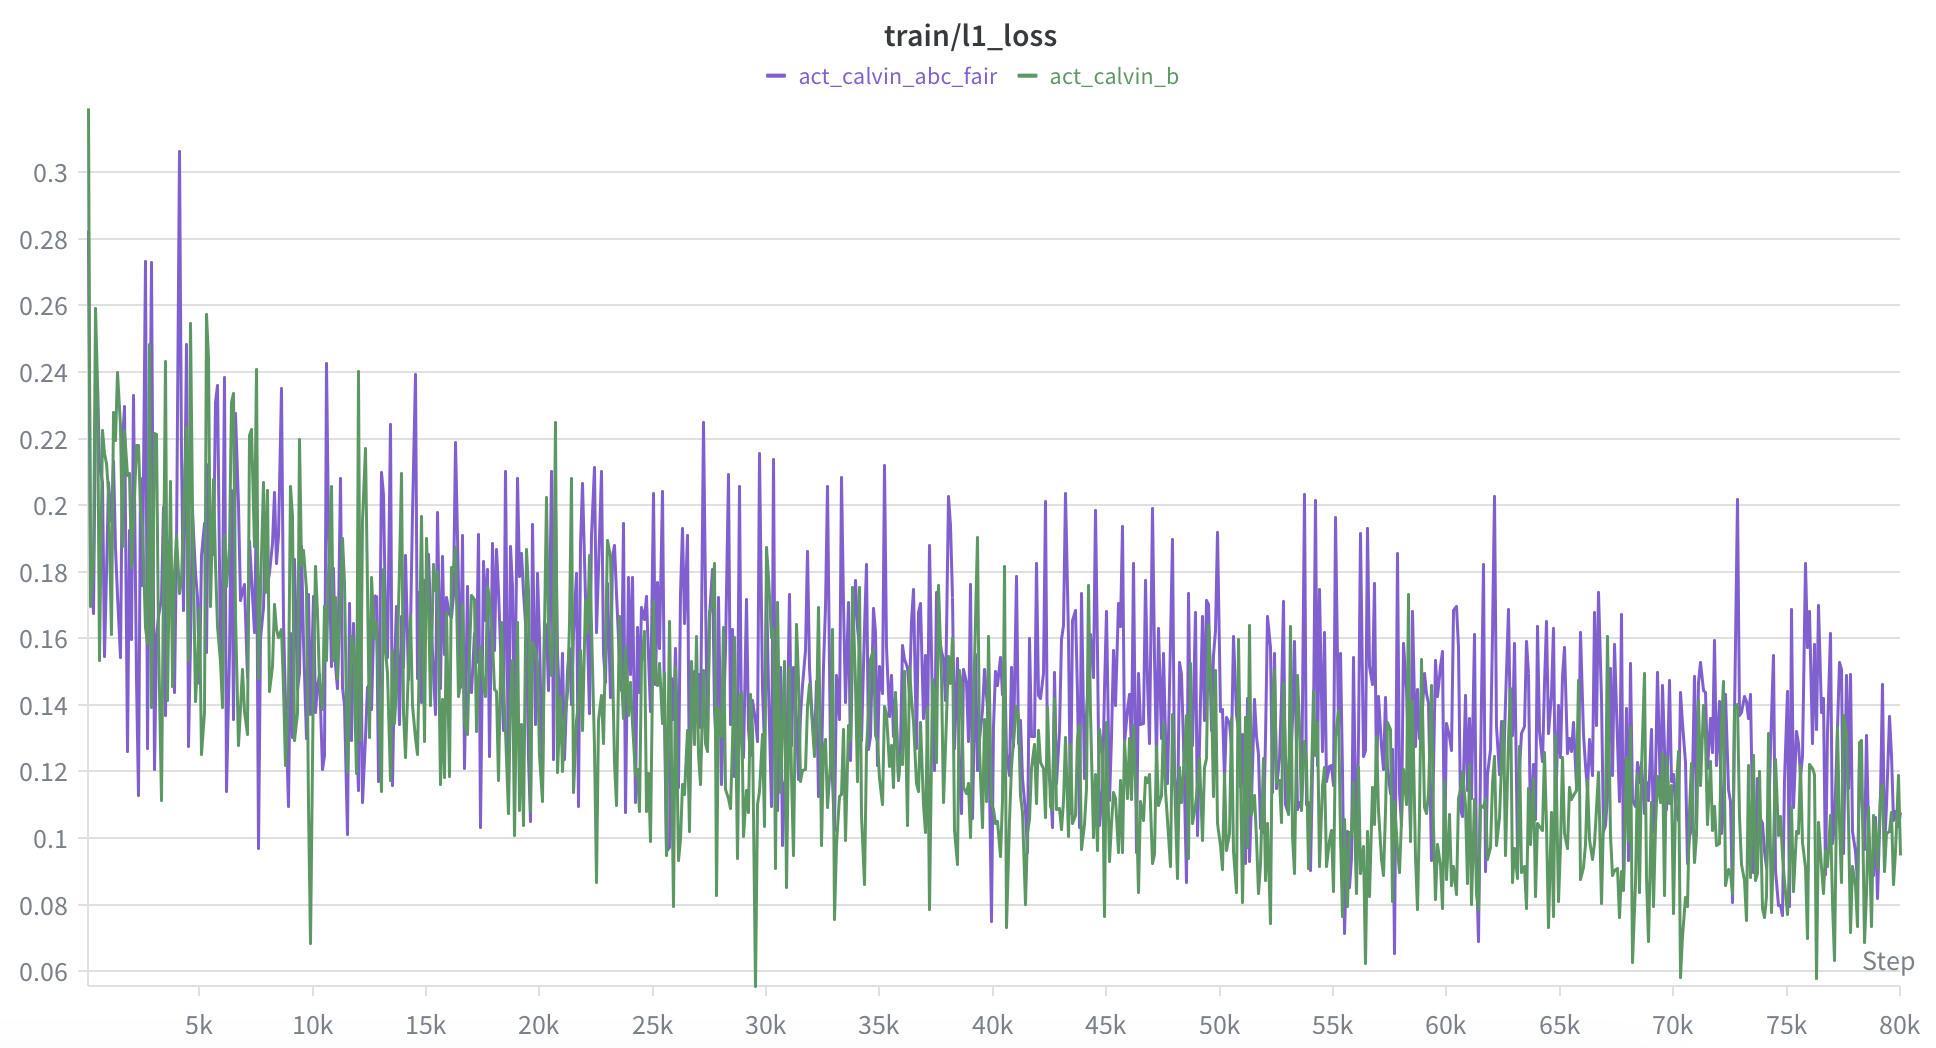
\includegraphics[width=\linewidth]{report_task2_figures/wandb_train_L1loss.png}
    \captionof{figure}{Action L1 loss}
    \label{fig:wandb-a}
  \end{minipage}\hfill
  \begin{minipage}[t]{0.24\textwidth}
    \centering
    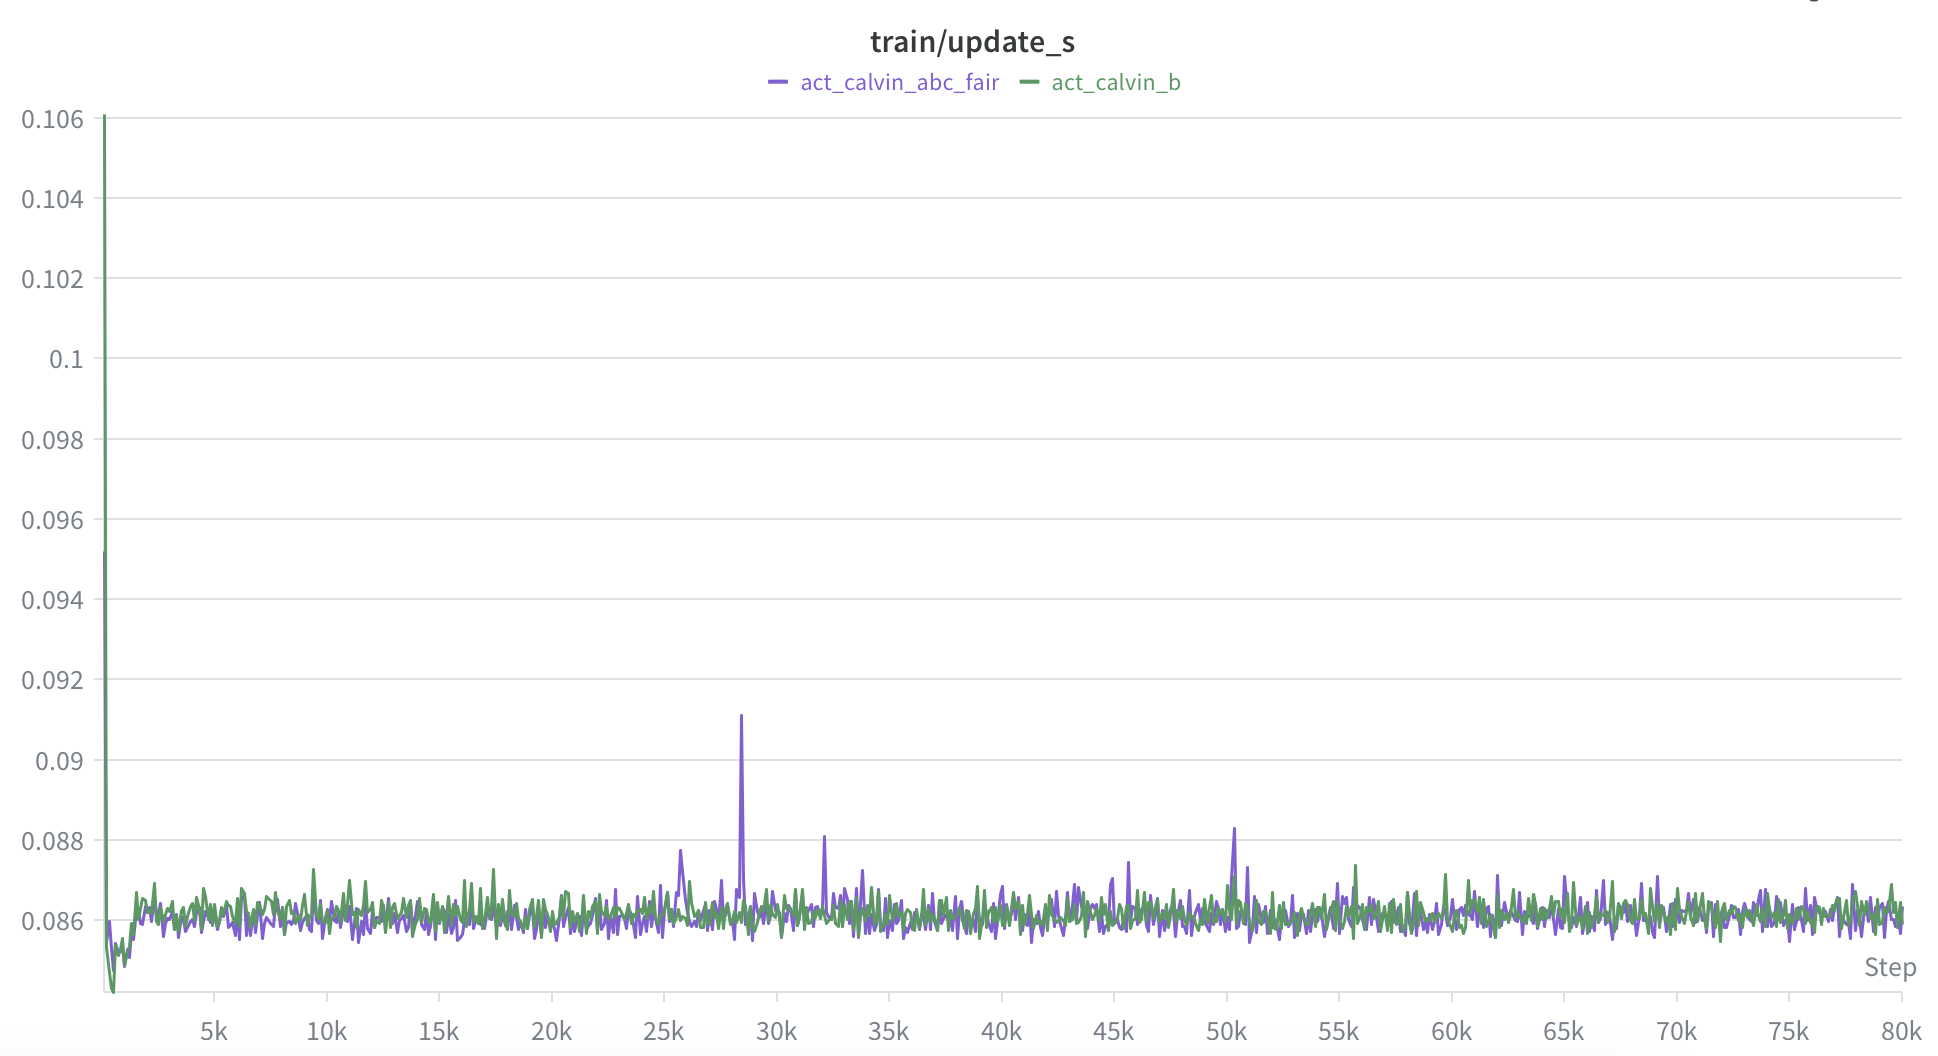
\includegraphics[width=\linewidth]{report_task2_figures/wandb_train_update_s.png}
    \captionof{figure}{Per-step update time}
    \label{fig:wandb-b}
  \end{minipage}\hfill
  \begin{minipage}[t]{0.24\textwidth}
    \centering
    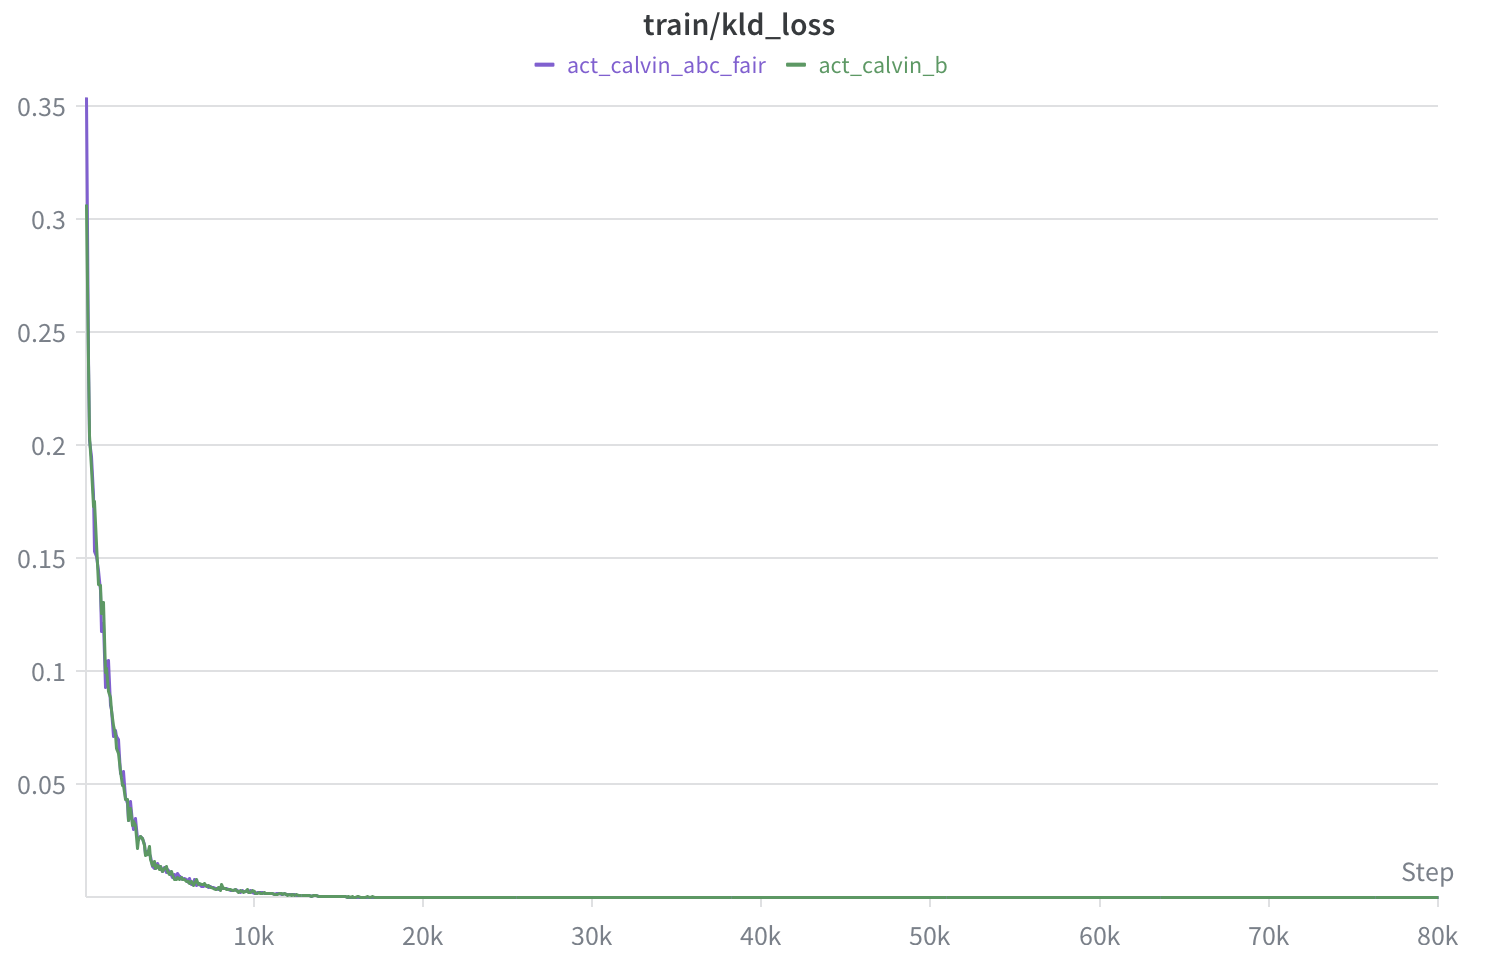
\includegraphics[width=\linewidth]{report_task2_figures/wandb_train_kld_loss.png}
    \captionof{figure}{KLD loss}
    \label{fig:wandb-c}
  \end{minipage}\hfill
  \begin{minipage}[t]{0.24\textwidth}
    \centering
    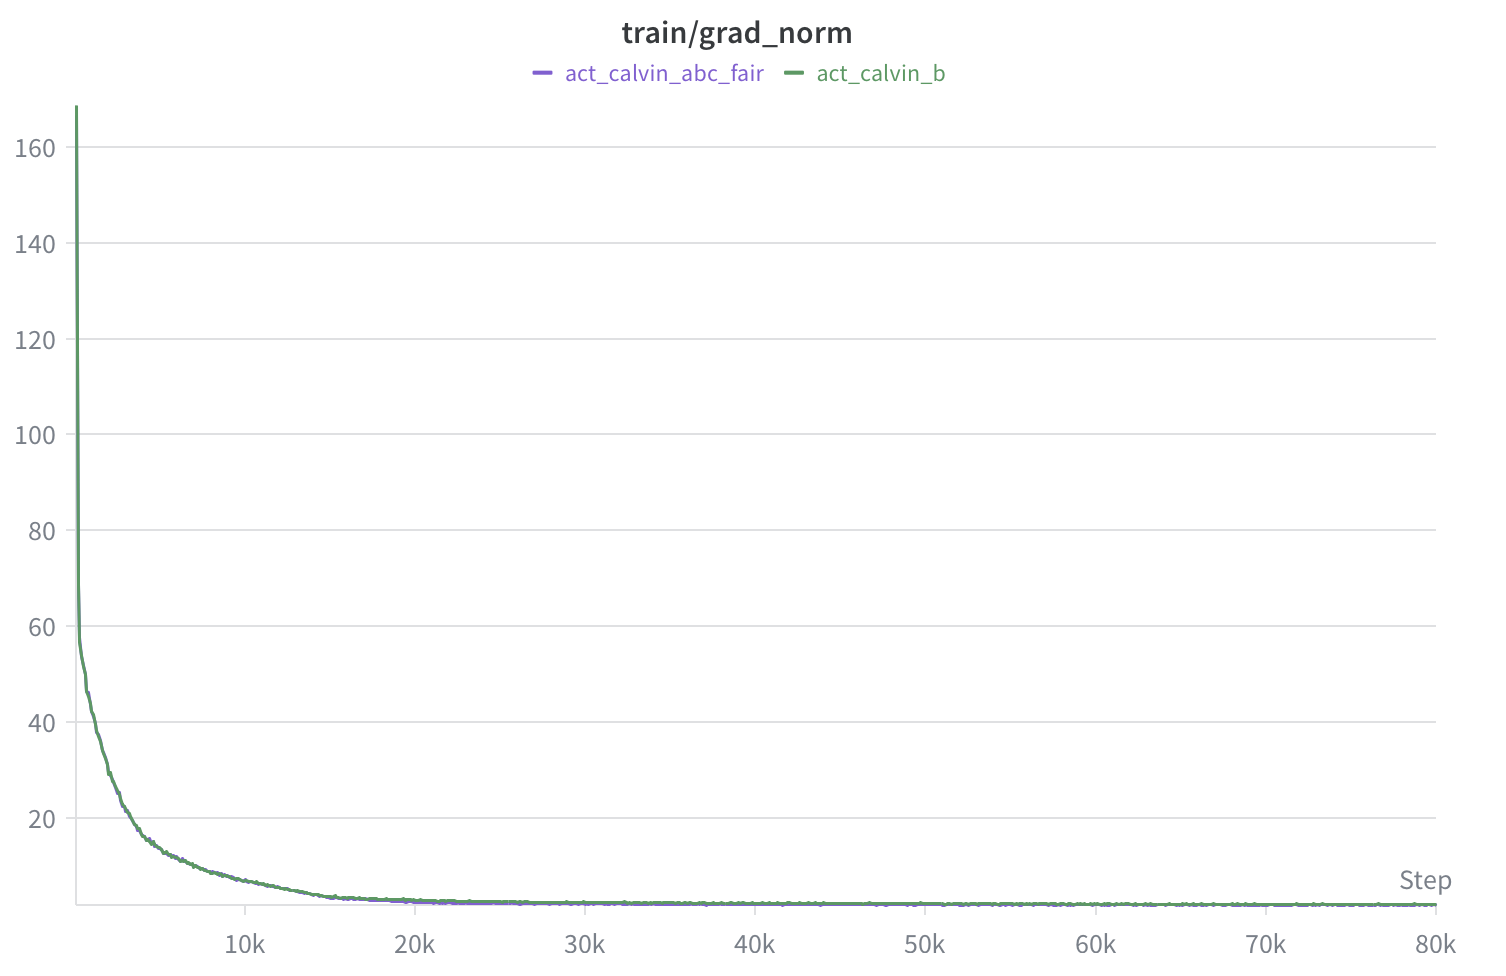
\includegraphics[width=\linewidth]{report_task2_figures/wandb_train_grad_norm.png}
    \captionof{figure}{Gradient norm}
    \label{fig:wandb-d}
  \end{minipage}
\end{figure*}

Fig.~\ref{fig:wandb-a}--\ref{fig:wandb-d} summarize L1, KLD, gradient norm, and update time over 80{,}000 gradient steps. Both experiments share identical \texttt{train\_config.json}; model, optimizer, seed, and step budget strictly aligned; sole variable is training environment coverage, so curve differences attribute entirely to data distribution breadth and diversity.

Early training (0--5k steps) KLD drops rapidly, pulling total loss down---ACT CVAE architecture: KLD constrains action latent posterior toward standard normal; initially far from prior, regularization dominates until $\sim$5k when KLD nears zero and L1 dominates action reconstruction.

\tabref{tab:train-milestones} shows from 10k steps ABC batch L1 exceeds B (0.17280 vs.\ 0.15011), matching data coverage: Exp-B completes 0.63 epoch with sufficient single-scene fit; Exp-ABC\_fair only 0.21 epoch with three visually distinct scenes and higher action variance.

\begin{table*}[!t]
  \centering
  \caption{Key training milestones}
  \label{tab:train-milestones}
  \footnotesize
  \setlength{\tabcolsep}{5pt}
  \begin{tabular}{@{}rcccccccccc@{}}
    \toprule
    Step & B L1 & ABC L1 & B loss & ABC loss & B epch & ABC epch & B KLD & ABC KLD & B grdn & ABC grdn \\
    \midrule
    100 & 0.31930 & 0.28268 & 3.38369 & 3.82084 & 0.01 & 0.00 & 0.306 & 0.354 & 168.8 & 166.6 \\
    5{,}000 & 0.16936 & 0.14646 & 0.27097 & 0.25971 & 0.32 & 0.11 & 0.0102 & 0.0113 & 13.80 & 13.53 \\
    10{,}000 & 0.15011 & 0.17280 & 0.17883 & 0.19123 & 0.63 & 0.21 & 0.00287 & 0.00184 & 6.92 & 7.08 \\
    20{,}000 & 0.12497 & 0.16011 & 0.12595 & 0.16079 & 1.22 & 0.41 & 0.00010 & 0.00007 & 2.82 & 2.43 \\
    40{,}000 & 0.10876 & 0.13371 & 0.10895 & 0.13387 & 2.36 & 0.79 & 0.000019 & 0.000016 & 2.21 & 1.94 \\
    60{,}000 & 0.08770 & 0.13451 & 0.08779 & 0.13463 & 3.55 & 1.18 & 0.000008 & 0.000011 & 2.03 & 1.88 \\
    80{,}000 & 0.09481 & 0.10770 & 0.09491 & 0.10777 & 4.77 & 1.59 & 0.000010 & 0.000007 & 1.96 & 1.79 \\
    \bottomrule
  \end{tabular}
  \tablenote{Note: loss computed per Eq.~(\ref{eq:loss}) from same-step L1 and KLD; L1 is normalized action-space chunk mean absolute error.}
\end{table*}

At 80k steps, training L1 is 0.09481 (B) / 0.10770 (ABC); B remains slightly lower but both gradient norms stabilize at $\sim$2, KLD near zero---both models converged stably. Fixed 80k checkpoint aligns gradient budget; subsequent generalization differences attribute to visual-action representation coverage of unseen environments, not convergence disparity; per-step update time is similar, excluding compute interference.

\subsection{In-Distribution Performance Analysis}

\begin{table}[H]
  \centering
  \caption{In-distribution vs.\ zero-shot L1 on env D}
  \label{tab:gap}
  \scriptsize
  \setlength{\tabcolsep}{2pt}
  \adjustbox{max width=\columnwidth}{%
  \begin{tabular}{@{}lcccc@{}}
    \toprule
    Train split & In-dist L1 & Zero-shot L1 (D) & Gap (abs.) & Gap (rel.) \\
    \midrule
    B & 0.310 & 0.522 & 0.212 & 1.68$\times$ \\
    ABC\_fair & 0.390 & 0.463 & 0.073 & 1.19$\times$ \\
    \bottomrule
  \end{tabular}}
\end{table}

\tabref{tab:gap} left columns: Exp-B $\mathcal{L}_{\mathrm{L1}}{=}0.310$ on \texttt{calvin\_env\_B}; Exp-ABC\_fair 0.390 on ABC mix, absolute gap 0.080. Offline full-frame eval 0.310/0.390 exceeds training batch L1 (80k: 0.095/0.108) because evaluation uses per-frame sliding replanning: each frame replans full chunk and accumulates error, adding open-loop prediction bias beyond single-chunk training loss.

0.390 should not be read as ``mixed training is worse''---difference reflects task difficulty, not model capability. ABC union spans three distinct desktop appearances, backgrounds, and layouts with higher action variance; ABC\_fair traverses only 1.59 epochs at 80k vs.\ B's 4.77 (\tabref{tab:train-milestones}).

\begin{table}[H]
  \centering
  \caption{L1 quantiles on in-dist and D}
  \label{tab:quantile}
  \footnotesize
  \begin{tabular}{@{}lcccc@{}}
    \toprule
    Train split & In-dist med. & D med. & In-dist $p_{90}$ & D $p_{90}$ \\
    \midrule
    B & 0.294 & 0.457 & 0.477 & 0.885 \\
    ABC\_fair & 0.360 & 0.411 & 0.614 & 0.769 \\
    \bottomrule
  \end{tabular}
\end{table}

\tabref{tab:quantile} shows ABC\_fair higher mean driven by right-tail hard frames ($p_{90}$ 0.614 vs.\ 0.477). These correspond to unusual viewpoints and poses rare in single-env data but more common in three-env mix.

Mechanism: single-env training has constant background/lighting/texture, enabling ``environment-specific background $\to$ action'' shortcuts without task-core features; multi-env training breaks shortcuts, forcing task-invariant features (arm pose, object spatial location), raising in-dist error but improving generalization potential. B has higher narrow-domain precision; ABC\_fair trades it for broader visual coverage.

\subsection{Zero-Shot Cross-Environment Generalization}

Applying same checkpoint to unseen environment D (267{,}373 frames) quantifies visual distribution shift impact. D differs systematically in table color, background layout, and lighting---typical OOD; performance drop reflects domain-invariance of visuomotor mapping.

\tabref{tab:gap}: Exp-B $\mathcal{L}_{\mathrm{L1}}{=}0.522$ on D, $\Delta_{\mathrm{abs}}{=}0.212$ (1.68$\times$); Exp-ABC\_fair 0.463, $\Delta_{\mathrm{abs}}{=}0.073$ (1.19$\times$), gap narrows $\sim$66\% relative to B. Single-env policy couples visual encoder to environment B statistics; shift to D causes domain bias propagating to action head.

In contrast, multi-env training exposes three distinct visual distributions, forcing invariant task features, reducing encoding bias and stabilizing predictions on D.

\begin{table}[H]
  \centering
  \caption{Proxy success rate $\mathrm{SR}_{0.5}$ on env D}
  \label{tab:sr}
  \footnotesize
  \begin{tabular}{@{}lcc@{}}
    \toprule
    Model & $\mathrm{SR}_{0.5}$ (D) & $\Delta$ vs.\ B \\
    \midrule
    B & 56.1\% & --- \\
    ABC\_fair & 66.4\% & +10.3 pp \\
    \bottomrule
  \end{tabular}
\end{table}

\tabref{tab:quantile} and \tabref{tab:sr} confirm tail behavior: B's D $p_{90}$ rises from 0.477 to 0.885 with many failure samples; ABC\_fair only to 0.769. $\mathrm{SR}_{0.5}$ on D rises from 56.1\% to 66.4\% (+10.3 pp)---substantive increase in successful frames, not mean-only optimization.

Fig.~\ref{fig:gapbar} shows classic ``crossover'': B lower in-dist but higher zero-shot---hallmark of improved generalization; lower narrow-distribution training error often accompanies environment overfitting and worse OOD performance.

\begin{figure}[H]
  \centering
  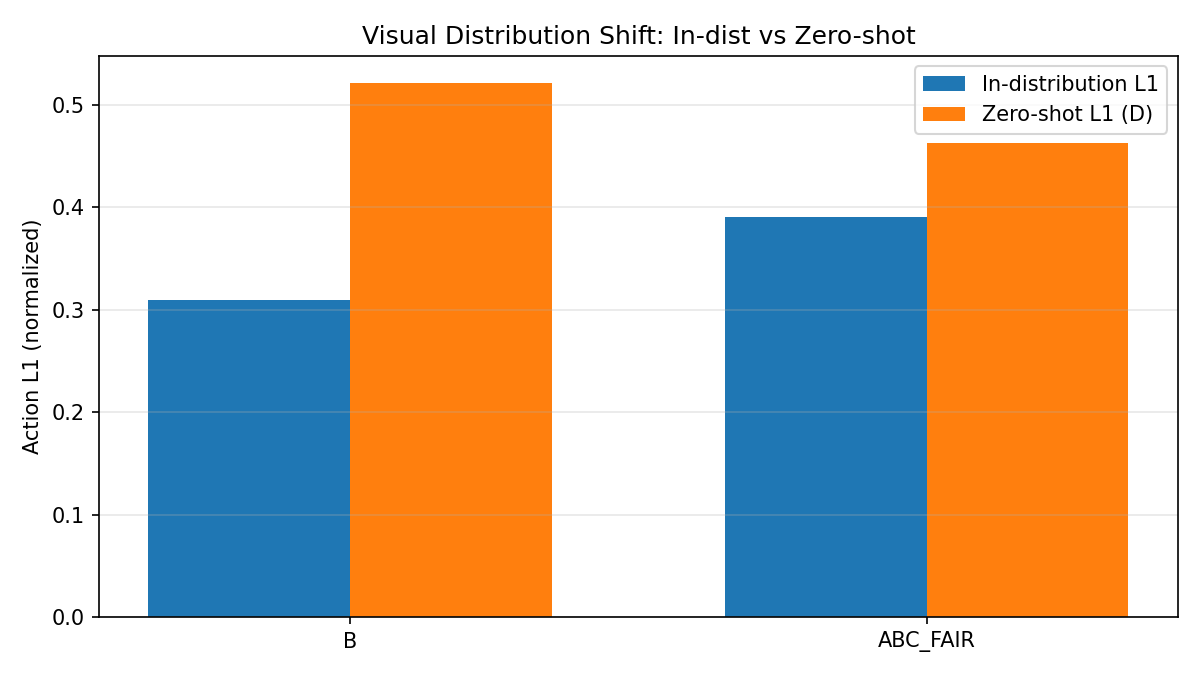
\includegraphics[width=\columnwidth]{report_task2_figures/gap_comparison.png}
  \caption{In-distribution vs.\ zero-shot mean L1 on env D. Left: Exp-B (0.310/0.522); right: Exp-ABC\_fair (0.390/0.463). Lower in-dist but higher zero-shot for B.}
  \label{fig:gapbar}
\end{figure}

\subsection{Action Dimension Decomposition}

Seven-dimensional decomposition verifies generalization mechanism: dimensions differ in visual dependence, so domain shift impact varies.

\begin{table}[H]
  \centering
  \caption{Per-dimension in-dist and D zero-shot L1}
  \label{tab:dim}
  \small
  \setlength{\tabcolsep}{4pt}
  \adjustbox{max width=\columnwidth}{%
  \begin{tabular}{@{}llccccccc@{}}
    \toprule
    Model & Split & pos\_x & pos\_y & pos\_z & rot\_x & rot\_y & rot\_z & gripper \\
    \midrule
    B & in-dist (B) & 0.253 & 0.252 & 0.300 & 0.532 & 0.456 & 0.268 & 0.115 \\
    B & zero-shot (D) & 0.527 & 0.516 & 0.571 & 0.651 & 0.665 & 0.480 & 0.327 \\
    ABC\_fair & in-dist (ABC) & 0.351 & 0.345 & 0.400 & 0.592 & 0.543 & 0.333 & 0.176 \\
    ABC\_fair & zero-shot (D) & 0.443 & 0.441 & 0.497 & 0.626 & 0.614 & 0.408 & 0.256 \\
    \bottomrule
  \end{tabular}}
\end{table}

\tabref{tab:dim}: Exp-B on D shows largest position dimension increases (pos\_x $\Delta{=}+0.274$) and significant gripper rise---position and gripper depend on spatially accurate vision; environment overfitting causes spatial errors under shift. Exp-ABC\_fair narrows position/gripper increments 60--70\%, core benefit being cross-scene spatial consistency.

rot\_x/rot\_y remain highest absolute error and main residual under shift in both experiments---rotation sensitive to texture, lighting, material reflection; multi-env training cannot fully eliminate this; rotation has higher DOF so small visual bias yields large angle error, bottleneck for cross-env generalization.

Dimension decomposition aligns with \S\ref{sec:chunking} chunk first-step gap (B: 0.149, ABC: 0.046): first step relies purely on current vision without action history inertia; gap reflects visual encoding domain bias.

%==============================================================================
\section{Action Chunking Robustness Under Visual Shift}
\label{sec:chunking}
%==============================================================================

This section analyzes chunk step-wise error $\bar{L}_k$ ($k{=}0,\ldots,64$) and step gaps $\Delta\bar{L}_k$ from \texttt{report\_B.json} and \texttt{report\_ABC\_FAIR.json}. Action Chunking is ACT's core: single forward pass outputs multi-step action block rather than per-frame single-step prediction, improving efficiency and temporal smoothness. Steps far from current observation are open-loop with accumulating error. Analyzing step curves under visual shift decouples: (1) visual domain shift raising baseline additively; (2) dynamics modeling defects causing temporal divergence ($\rho$). This distinction is central to cross-environment robustness and chunking utility.

\subsection{Quantitative Shape of Chunk Step-Wise Error}

\tabref{tab:chunkdeg} and Fig.~\ref{fig:chunk-b}, \ref{fig:chunk-abc}: visual shift mainly raises $\bar{L}_k$ baseline in parallel; horizon degradation $\rho=\bar{L}_{64}/\bar{L}_0$ nearly unchanged between in-dist and D (B: 1.49$\to$1.51; ABC: 1.58$\to$1.57).

\begin{table}[H]
  \centering
  \caption{Chunk L1 and horizon degradation $\rho$}
  \label{tab:chunkdeg}
  \footnotesize
  \adjustbox{max width=\columnwidth}{%
  \begin{tabular}{@{}lcccccc@{}}
    \toprule
    Exp & $\bar{L}_0$ (in) & $\bar{L}_{64}$ (in) & $\rho$ (in) & $\bar{L}_0$ (D) & $\bar{L}_{64}$ (D) & $\rho$ (D) \\
    \midrule
    B & 0.341 & 0.509 & 1.49 & 0.490 & 0.741 & 1.51 \\
    ABC\_fair & 0.389 & 0.616 & 1.58 & 0.434 & 0.682 & 1.57 \\
    \bottomrule
  \end{tabular}}
\end{table}

\begin{figure}[H]
  \centering
  \begin{minipage}[t]{0.48\columnwidth}
    \centering
    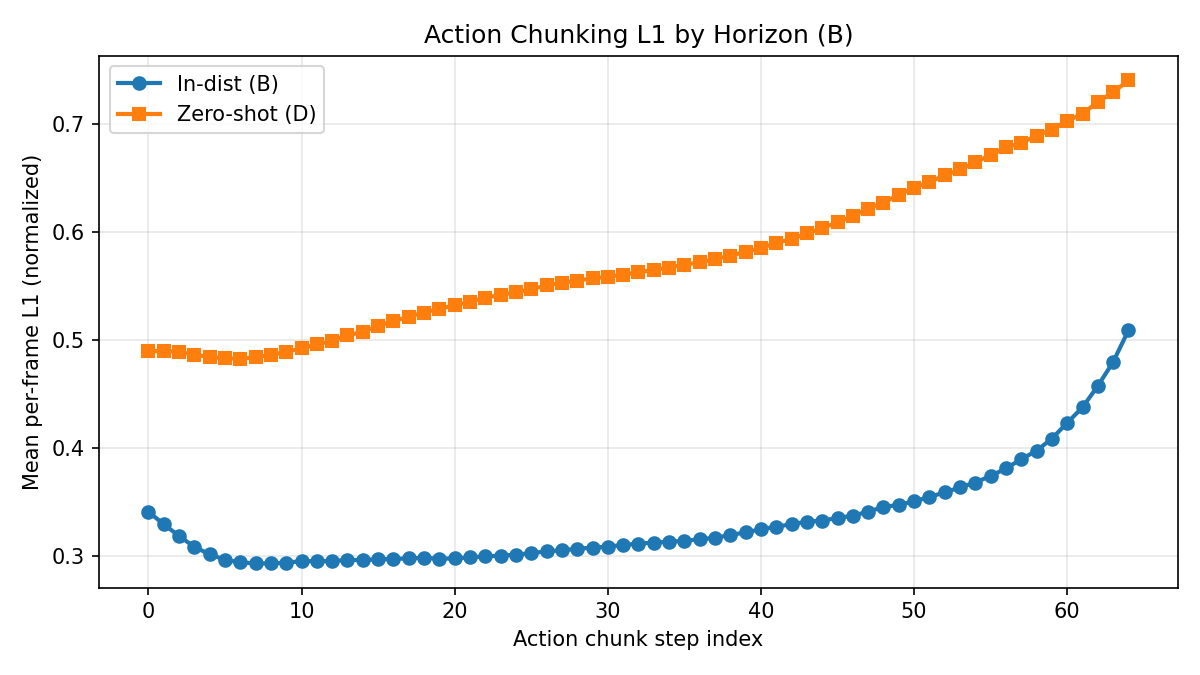
\includegraphics[width=\linewidth]{report_task2_figures/chunk_l1_B.png}
    \captionof{figure}{Chunk-step mean L1 $\bar{L}_k$ ($k{=}0,\ldots,64$), Exp-B. $\max_k\Delta\bar{L}_k{=}0.297$ ($k{=}56$). Dashed: $k{=}9$.}
    \label{fig:chunk-b}
  \end{minipage}\hfill
  \begin{minipage}[t]{0.48\columnwidth}
    \centering
    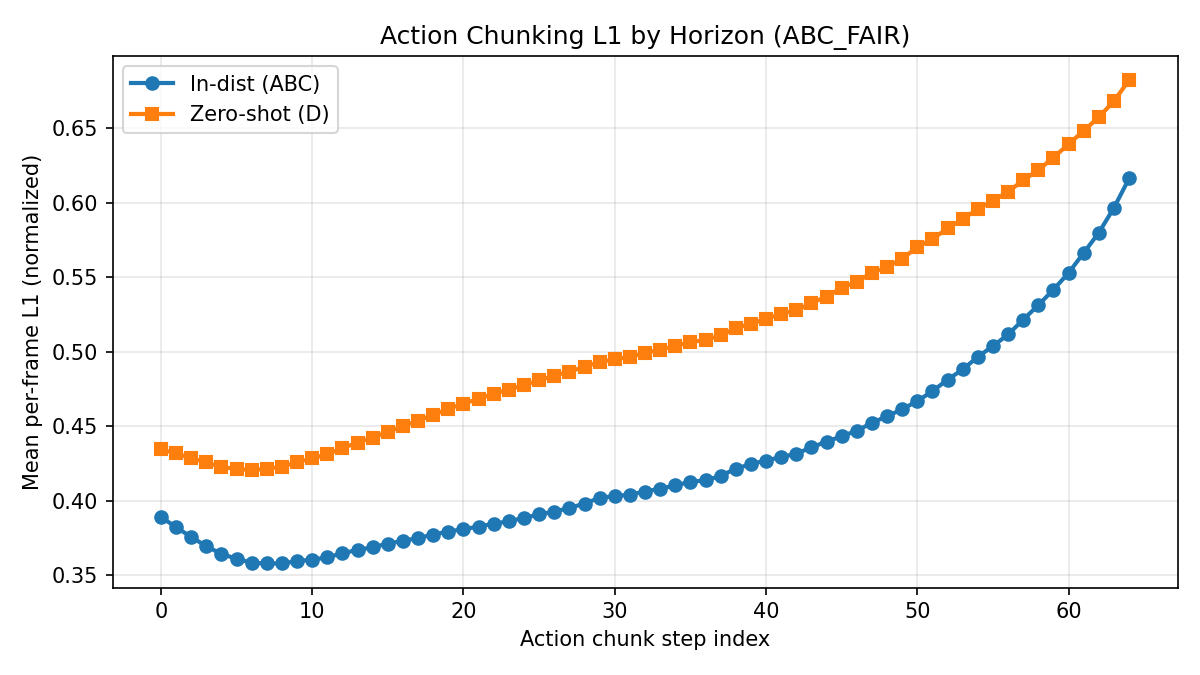
\includegraphics[width=\linewidth]{report_task2_figures/chunk_l1_ABC_FAIR.png}
    \captionof{figure}{Chunk-step mean L1 $\bar{L}_k$ ($k{=}0,\ldots,64$), Exp-ABC\_fair. $\max_k\Delta\bar{L}_k{=}0.103$ ($k{=}50$). Dashed: $k{=}9$.}
    \label{fig:chunk-abc}
  \end{minipage}
\end{figure}

Mechanism: degradation ratio $\rho$ reflects temporal dynamics modeling quality, independent of visual domain shift. Step 0 ($k=0$) uses current observation; later steps are open-loop extrapolation from internal dynamics prior; visual shift only affects encoding baseline, not relative degradation rate. Cross-environment visual shift adds baseline error, not multiplicative temporal divergence---core evidence for ACT chunking cross-env robustness.

B in-dist maintains low-error plateau $k{=}0$--35 ($\bar{L}_k{\approx}0.29$--0.31), rising after $k{>}40$ to 0.509. Early chunk steps constrained by accurate vision; beyond step 40 open-loop bias accumulates. On D, curve rises monotonically from $\bar{L}_0{=}0.490$ without in-dist plateau---visual shift eliminates observation-supported low-error region.

ABC\_fair D orange line parallels in-dist blue with stable gap throughout; at $k{=}50$ gap only 0.103, 35\% of B peak 0.297. Cross-scale confirmation of frame-level findings: multi-env training lowers initial state estimation bias, shifting entire $\bar{L}_k$ curve down without changing degradation rate. \apptabref{apptab:chunk-steps} B peak $\Delta\bar{L}_k$ $\sim$3.1$\times$ ABC, same order as frame-level $\Delta_{\mathrm{abs}}$.

Deployment uses sliding-window replanning: execute subset of chunk then replan. At 30\,Hz, $k{=}10$ is $\sim$0.33\,s interval: B on D $\bar{L}_{0:9}{\approx}0.487$, ABC ${\approx}0.427$, both manageable; at $k{=}20$, B $\bar{L}_{19}^{\mathrm{D}}{=}0.529$ exceeds safe threshold. Multi-env training supports longer replan intervals at lower compute with maintained precision.

%==============================================================================
\section{Discussion}
%==============================================================================

\subsection{Core Findings and Literature Comparison}

Strictly fixing ACT architecture, optimizer, gradient steps, and seed isolates ``training data distribution breadth'' as sole variable with clear causal attribution. Three mechanistic layers compare with literature.

First, low in-distribution loss does not predict unseen-domain performance; visual shortcut overfitting is endemic to end-to-end policies. B achieves lower in-dist L1 (0.310 vs.\ 0.390) but worse zero-shot with 66\% gap reduction for ABC---consistent with Codevilla et al.\cite{codevilla2019exploring} on autonomous driving: policies capture superficial visual shortcuts (table texture, background color) that fail OOD. Our domain shift is tabletop layout/lighting, not city-scale, yet in-dist vs.\ generalization decoupling still appears---universal whenever learning pixel-to-action from narrow distribution.

Second, multi-environment training expands visual support set---natural domain randomization. ABC mixes three environments, forcing domain-invariant task features; logic aligns with Tobin et al.\cite{tobin2017domain} but uses real scene diversity rather than synthetic random textures. Marginal effect remains: ABC on D (0.463) still exceeds in-dist (0.390); three environments do not fully cover D statistics.

Third, action chunking exhibits visual-temporal decoupling---underexplored robustness source. $\rho\approx1.5$ stable across in-dist and zero-shot; visual shift parallel-shifts $\bar{L}_k$ baseline without changing degradation slope. Mixed training reduces max step gap 0.297 ($k{=}56$) to 0.103 ($k{=}50$). Two-layer structure: visual encoder maps images to state features (domain-shift sensitive, sets baseline); action decoder generates chunk from latent dynamics (domain-invariant, sets degradation rate). Optimization for cross-env robustness should focus on visual domain invariance, not chunk temporal structure.

Dimension decomposition: rotation (rot\_x/rot\_y) bottleneck; position/gripper benefit most---geometric vs.\ appearance feature hierarchy: spatial relations are stable cross-env; rotation depends on texture/lighting detail. Aligns with ``geometry more domain-invariant than appearance'' in computer vision.

\subsection{Limitations and Future Work}

Three limitations: (1) all metrics offline open-loop frame-averaged; $\mathrm{SR}_\tau$ not equivalent to CALVIN closed-loop long-horizon success---needs simulation validation. (2) aligned on gradient steps not epochs; ABC 1.59 epochs may underfit, confounding in-dist error. (3) CALVIN simulation only; no backbone/augmentation ablation; sim2real untested.

Future: (1) CALVIN PyBullet for task-level success; (2) epoch-aligned ABC retraining plus single-env A/C controls; (3) scan chunk length vs.\ replan window for deployment tradeoffs; (4) quaternion rotation or geometric priors for rotation bottleneck.

%==============================================================================
\section{Conclusion}
%==============================================================================

Controlled experiments systematically examine training data breadth effects on ACT cross-environment generalization, with chunk step-wise and dimension decomposition revealing mechanism. Three conclusions:

First, data distribution breadth is core to generalization; in-dist error is insufficient for cross-scene model selection. Single-env lower fit error reflects environment overfitting; multi-env excels on unseen D, compressing gap from 0.212 (1.68$\times$) to 0.073 (1.19$\times$), $\mathrm{SR}_{0.5}$ 56.1\%$\to$66.4\%. ``Breadth for zero-shot robustness'': $\sim$0.08 in-dist cost for cross-visual stability.

Second, ACT chunking robustness from visual-temporal decoupling; optimization focus is visual side. Visual shift raises baseline without changing $\rho\approx1.5$ degradation---action temporal dynamics are domain-invariant; bottleneck is visual state estimation. Multi-env training improves visual invariance, synchronously lowering entire chunk error.

Third, dimensional generalization heterogeneity: position/gripper gain 60\%+ cross-env error reduction; rotation remains bottleneck due to appearance-dependent features. Future rotation tasks need specialized representation beyond data scaling.

Overall, multi-env training improves embodied policy generalization; chunk step analysis and dimension decomposition reveal where gains act, guiding ACT cross-scene deployment and algorithm optimization.

%==============================================================================
{\small
\begin{thebibliography}{99}
%==============================================================================

\bibitem{schoenberger2016sfm}
Sch\"onberger, J. L. and Frahm, J.-M.
\newblock Structure-from-motion revisited.
\newblock In \emph{CVPR}, 2016.

\bibitem{schoenberger2016mvs}
Sch\"onberger, J. L., et al.
\newblock Pixelwise view selection for unstructured multi-view stereo.
\newblock In \emph{ECCV}, 2016.

\bibitem{mildenhall2020nerf}
Mildenhall, B., et al.
\newblock NeRF: Representing scenes as neural radiance fields for view synthesis.
\newblock In \emph{ECCV}, 2020.

\bibitem{barron2021mipnerf}
Barron, J. T., et al.
\newblock Mip-NeRF: A multiscale representation for anti-aliasing neural radiance fields.
\newblock In \emph{ICCV}, 2021.

\bibitem{barron2022mipnerf360}
Barron, J. T., et al.
\newblock Mip-NeRF 360: Unbounded anti-aliased neural radiance fields.
\newblock In \emph{CVPR}, 2022.

\bibitem{muller2022instantngp}
M\"uller, T., et al.
\newblock Instant neural graphics primitives with a multiresolution hash encoding.
\newblock \emph{ACM TOG}, 41(4), 2022.

\bibitem{kerbl2023gaussians}
Kerbl, B., et al.
\newblock 3D Gaussian splatting for real-time radiance field rendering.
\newblock \emph{ACM TOG}, 42(4), 2023.

\bibitem{huang20242dgs}
Huang, B., et al.
\newblock 2D Gaussian splatting for geometrically accurate radiance fields.
\newblock In \emph{SIGGRAPH}, 2024.

\bibitem{poole2022dreamfusion}
Poole, B., et al.
\newblock DreamFusion: Text-to-3D using 2D diffusion.
\newblock In \emph{ICLR}, 2023.

\bibitem{lin2023magic3d}
Lin, C.-H., et al.
\newblock Magic3D: High-resolution text-to-3D content creation.
\newblock In \emph{CVPR}, 2023.

\bibitem{wang2023prolificdreamer}
Wang, Z., et al.
\newblock ProlificDreamer: High-fidelity and diverse text-to-3D generation with variational score distillation.
\newblock In \emph{NeurIPS}, 2023.

\bibitem{qian2023magic123}
Qian, G., et al.
\newblock Magic123: One image to high-quality 3D object generation using both 2D and 3D diffusion priors.
\newblock In \emph{ICLR}, 2024.

\bibitem{liu2023zero123}
Liu, R., et al.
\newblock Zero-1-to-3: Zero-shot one image to 3D object.
\newblock In \emph{ICCV}, 2023.

\bibitem{threestudio2023}
Ye, T., et al.
\newblock threestudio: A unified framework for 3D content generation.
\newblock \url{https://github.com/threestudio-project/threestudio}, 2023.

\bibitem{rombach2022ldm}
Rombach, R., et al.
\newblock High-resolution image synthesis with latent diffusion models.
\newblock In \emph{CVPR}, 2022.

\bibitem{ross2011dagger}
Ross, S., Gordon, G., and Bagnell, D.
\newblock A reduction of imitation learning and structured prediction to no-regret online learning.
\newblock In \emph{AISTATS}, 2011.

\bibitem{codevilla2019exploring}
Codevilla, F., M\"uller, A., L\'opez, A., Koltun, V., and Dosovitskiy, A.
\newblock Exploring the limitations of behavior cloning in autonomous driving.
\newblock In \emph{ICCV}, 2019.

\bibitem{dehaan2019causal}
De Haan, P., Jayaraman, D., and Levine, S.
\newblock Causal confusion in imitation learning.
\newblock In \emph{NeurIPS}, 2019.

\bibitem{tobin2017domain}
Tobin, J., et al.
\newblock Domain randomization for transferring deep neural networks from simulation to the real world.
\newblock In \emph{IROS}, 2017.

\bibitem{zhao2023learning}
Zhao, T. Z., Kumar, V., Levine, S., and Finn, C.
\newblock Learning fine-grained bimanual manipulation with low-cost hardware.
\newblock In \emph{RSS}, 2023. arXiv:2304.13705.

\bibitem{mees2022calvin}
Mees, O., Hermann, L., Rosete-Beas, E., and Burgard, W.
\newblock CALVIN: A benchmark for language-conditioned policy learning for long-horizon robot manipulation tasks.
\newblock \emph{IEEE Robotics and Automation Letters}, 7(3):7327--7334, 2022.

\bibitem{cadene2024lerobot}
Cad\`ene, R., et al.
\newblock LeRobot: State-of-the-art machine learning for real-world robotics in PyTorch.
\newblock \url{https://github.com/huggingface/lerobot}, 2024.

\bibitem{lerobot2025datasetv3}
Hugging Face LeRobot Team.
\newblock LeRobotDataset v3.0 documentation.
\newblock \url{https://huggingface.co/docs/lerobot/lerobot-dataset-v3}, 2025.

\end{thebibliography}
}

\clearpage
\appendix
\renewcommand{\appendixname}{Appendix}
\renewcommand{\thesection}{\Alph{section}}
\begin{center}
  {\Large\bfseries Appendix}
\end{center}
\vspace{0.6em}
\section{Submission Information and Reproducibility}

\subsection{Code Repository and Data Cloud Storage}

GitHub repository (Task 1 and Task 2): \url{https://github.com/daomuyang/CV_Final_Liesen_Gai/tree/main}

Baidu Netdisk link: \url{https://pan.baidu.com/s/1dlkCUwM8b2_L2cgbFi3RKA?pwd=stq2}\\
Extraction code: \texttt{stq2}

Cloud storage includes Task 1 \texttt{submission\_assets/} ($\sim$8.8\,GB), \texttt{third\_party/} ($\sim$200\,MB, including 2DGS, COLMAP, Magic123, threestudio); and Task 2 LeRobot datasets and checkpoints. GitHub contains code, scripts, and \texttt{outputs/} evaluation logs.

\subsection{Task 1: Multi-Object 3D Reconstruction and AIGC Scene Fusion}
\label{sec:t1-repro}
%==============================================================================

\subsubsection{Directory Structure}

GitHub repository \texttt{task1/} structure (excluding cloud-provided \texttt{submission\_assets/} and \texttt{third\_party/}):
\begin{lstlisting}
task1/
|-- README.md
|-- environment.yml              # Conda environment (task1)
|-- patches/                     # Patches for third-party libraries
|   |-- 2d-gaussian-splatting-alpha-mask.patch
|   `-- Magic123-wandb.patch
|-- scripts/
|   |-- common.sh                # Path constants, shared functions
|   |-- setup_server.sh          # Server environment setup
|   |-- timing.sh                # Wall-clock timing
|   |-- wandb.sh                 # WandB offline logging
|   |-- pipeline/                # Four pipeline entry points
|   |   |-- object_a.sh          # Object A: COLMAP + 2DGS
|   |   |-- object_b.sh          # Object B: threestudio SDS
|   |   |-- object_c.sh          # Object C: Magic123
|   |   `-- background.sh        # Background: garden + 2DGS
|   `-- tools/
|       |-- preprocess_image.py
|       |-- plot_magic123_loss.py
|       |-- log_metrics_to_wandb.py
|       |-- blender_vertex_color.py
|       `-- run_blender_color.sh
`-- outputs/
    |-- timing.csv               # Per-stage wall-clock time
    `-- data/                    # Training metric CSVs (report/WandB)
        |-- twodgs:*.csv
        |-- dreamfusion:loss_*.csv
        `-- magic123:loss_*.csv
\end{lstlisting}

Cloud third\_party/ contains 2d-gaussian-splatting,\\ colmap, Magic123, threestudio.Cloud submission\\\_assets/ structure:
\begin{lstlisting}
submission_assets/
|-- object_A/                         # Sneaker · COLMAP + 2DGS (10000 iter)
|   |-- images_raw/                   # 36 self-captured raw images
|   |-- images/                       # Matted foreground
|   |-- sparse/                       # COLMAP sparse reconstruction
|   |-- database.db
|   `-- 2dgs_output/
|       |-- train/ours_10000/         # fuse_post.ply, vis/, renders/, gt/
|       `-- point_cloud/iteration_10000/
|-- object_B/                         # Plush puppy · threestudio SDS (12000 iter)
|   |-- ckpts/last.ckpt
|   |-- configs/parsed.yaml, raw.yaml
|   |-- csv_logs/
|   |-- cmd.txt
|   |-- tb_logs/
|   `-- save/
|       |-- it12000-export/           # model.obj + model.mtl + texture_kd.jpg
|       |-- it12000-0.png, it12000-test.mp4
|       `-- it{step}-0.png           # Training preview frames
|-- object_C/                         # Guitar · Magic123 (coarse/fine 5000 iter each)
|   |-- images/                       # 0001.jpg, rgba.png, etc.
|   `-- magic123_output/
|       |-- object_C_coarse/          # mesh/, checkpoints/, run/, training/, validation/, results/
|       `-- object_C_fine/
|-- garden/                           # Mip-NeRF 360 background · 2DGS (10000 iter)
|   |-- images/, images_2/, images_4/, images_8/
|   |-- sparse/, poses_bounds.npy
|   `-- 2dgs_output/
|       |-- train/ours_10000/         # fuse_unbounded_post.ply, vis/, renders/, gt/
|       `-- point_cloud/iteration_10000/
|-- scene_compose.blend               # Blender fusion project
`-- wandering.mov                     # Orbit wandering video
\end{lstlisting}

Data directory conventions in \apptabref{apptab:t1-repro-layout}. Training curves, validation metrics, and wall-clock times in the main text are drawn from GitHub repository logs; data sources are summarized as follows:
\begin{itemize}[nosep,leftmargin=*]
  \item \textbf{Wall-clock timing}: \texttt{task1/outputs/timing.csv}, fields \texttt{object, stage, elapsed\_seconds, exit\_status}, recording per-stage wall-clock time; Object A full log includes two preprocessing+COLMAP runs (847\,s total); main-text summaries use the final successful path.
  \item \textbf{2DGS training/validation metrics}:\\ \texttt{task1/outputs/data/twodgs:loss\_total.csv}, \texttt{twodgs\_loss\_normal.csv},twodgs:evl\_psnr.csv, \texttt{twodgs:evl\_l1\_losscsv.csv}, for Object A and garden background loss curves and hold-out PSNR/L1.
  \item \textbf{SDS training metrics}: \texttt{task1/outputs/data/dream\\-fusion:loss\_sds.csv},loss\_opaque.csv, \texttt{loss\_orient.csv}, \texttt{loss\_sparsity.csv}, for Object B four loss curves; step 11999 values additionally from cloud \texttt{object\_B/csv\_logs/version\_0/metrics.csv}.
  \item \textbf{Magic123 training metrics}: \texttt{task1/outputs/data/\\magic123:loss\_total.csv},loss\_rgb.csv,loss\_mask.csv,for Object C coarse/fine stage-wise losses.
  \item \textbf{Render and mesh outputs}: cloud \texttt{submission\\\_assets/} per-object training directories (paths in \apptabref{apptab:t1-repro-layout} note).
\end{itemize}

\subsubsection{Environment and Execution}

On server, run \texttt{scripts/setup\_server.sh}, activate Conda env \texttt{task1}, then run four pipeline scripts sequentially. WandB optional offline mode. Blender vertex-color script at \texttt{scripts/tools/run\_blender\_color.sh}. Full commands in README.

\subsubsection{Datasets and Reproduction Steps}

All inputs/outputs in \texttt{submission\_assets/}; third-party libs in \texttt{third\_party/} (2DGS, COLMAP, Magic123, threestudio). GitHub has code and \texttt{outputs/} logs only. Pipelines read/write via \texttt{DATASET\_ROOT=submission\_assets/}, \texttt{THIRD\_PARTY\_DIR=third\_party/} in \texttt{scripts/common.sh}. Extract \texttt{submission\_assets/} and \texttt{third\_party/} from cloud to \texttt{task1/}, preserving \texttt{object\_A/}, \texttt{object\_B/}, \texttt{object\_C/}, \texttt{garden/} subdirectories.

Reproduction steps:
\begin{enumerate}
  \item \texttt{git clone} repository, \texttt{bash scripts/setup\_server.sh}, \texttt{conda activate task1}
  \item Extract \texttt{submission\_assets/}, \texttt{third\_party/} from cloud to \texttt{task1/}
  \item Run four pipeline scripts sequentially:
  \begin{itemize}[nosep,leftmargin=*]
    \item \texttt{bash scripts/pipeline/object\_a.sh}
    \item \texttt{bash scripts/pipeline/object\_b.sh}
    \item \texttt{bash scripts/pipeline/object\_c.sh}
    \item \texttt{bash scripts/pipeline/background.sh}
  \end{itemize}
\end{enumerate}

View results only: after cloud extraction, open \texttt{scene\_compose.blend} and \texttt{wandering.mov}, or inspect mesh paths in \apptabref{apptab:t1-repro-layout} note without retraining.

\subsection{Task 2: LeRobot ACT Cross-Environment Generalization}
\label{sec:repro}
%==============================================================================

\subsubsection{Repository Contents}

Repository includes full train/eval scripts, environment configs, WandB training curve screenshots (\texttt{wandb\_train\_*.png}), \texttt{grad\_norm.csv}, \texttt{kld\_loss.csv}, and eval JSON/figures. Virtual environment not uploaded; rebuild per below.

\subsubsection{Datasets and Model Weights}

Task 2 data and checkpoints share cloud link above. Cloud contains five LeRobot v3.0 dataset dirs (\texttt{calvin\_env\_\{A,B,C,ABC,D\}}) and two best checkpoints (\texttt{outputs/train\_b/checkpoints/080000}, \texttt{outputs/train\_abc\_fair/checkpoints/080000}). Place data in \texttt{task2/data/}, merge weights into GitHub \texttt{task2/outputs/} (do not overwrite eval JSON). Each \texttt{pretrained\_model/} must contain all 7 files (\texttt{model.safetensors}, \texttt{config.json}, \texttt{train\_config.json}, preprocessor/postprocessor JSON and safetensors). If only \texttt{080000/} exists, create symlinks before eval:
\begin{lstlisting}
ln -sfn 080000 outputs/train_b/checkpoints/last
ln -sfn 080000 outputs/train_abc_fair/checkpoints/last
\end{lstlisting}

\subsubsection{Environment Configuration}

\textbf{GPU server}
\begin{lstlisting}
cd task2
bash scripts/setup_server.sh    # reads environment.yml
conda activate task2
python scripts/verify_dataset.py
\end{lstlisting}

\textbf{Server venv alternative}
\begin{lstlisting}
cd task2
python3.12 -m venv .venv && source .venv/bin/activate
pip install -U pip wheel
pip install torch==2.10.0 torchvision==0.25.0 \
  --index-url https://download.pytorch.org/whl/cu121
pip install -r requirements-server.txt
export HF_HUB_OFFLINE=1
\end{lstlisting}

\textbf{macOS local smoke test}
\begin{lstlisting}
bash scripts/setup_local.sh && source .venv/bin/activate
bash scripts/run_smoke.sh
\end{lstlisting}

Environment: Python 3.12, PyTorch 2.10.0 (CUDA 12.1), LeRobot 0.5.1, seed \texttt{SEED=42}. Configs in \texttt{environment.yml} (server), \texttt{environment-local.yml} (local).

\subsubsection{Training and Evaluation Commands}

\begin{lstlisting}
export SEED=42
# Training (~2 hours each, 80k steps)
bash scripts/train.sh B server
bash scripts/train.sh ABC_fair server
# Offline eval + report (no retraining)
bash scripts/eval_report.sh B server
bash scripts/eval_report.sh ABC_fair server
bash scripts/eval_compare.sh B ABC_fair
# Zero-shot -> D
bash scripts/eval_zeroshot.sh B server
bash scripts/eval_zeroshot.sh ABC_fair server
\end{lstlisting}

WandB offline logs at \texttt{outputs/train\_*/wandb/}, upload via \texttt{wandb sync}. Main eval artifacts: \texttt{outputs/report\_*.json}, \texttt{outputs/eval\_*\_on\_*.json}, \texttt{outputs/gap\_comparison.png}.

\subsubsection{Directory Structure}

\begin{lstlisting}
task2/
|-- README.md                 # Documentation
|-- environment.yml           # GPU server conda env
|-- environment-local.yml     # macOS local smoke conda env
|-- environment-server.yml    # Same as environment.yml
|-- requirements-server.txt   # Server pip deps (lerobot, etc.)
|-- requirements-local.txt    # Local pip deps
|-- grad_norm.csv             # WandB export train/grad_norm (B & ABC_fair)
|-- kld_loss.csv              # WandB export train/kld_loss (B & ABC_fair)
|-- data/                     # Datasets (see Data Preparation)
|   |-- calvin_env_A/
|   |-- calvin_env_B/
|   |-- calvin_env_C/
|   |-- calvin_env_ABC/
|   `-- calvin_env_D/
|-- scripts/                  # Train / eval scripts
|   |-- setup_server.sh       # Server one-click env setup
|   |-- setup_local.sh        # macOS local env setup
|   |-- verify_dataset.py     # Data validation
|   |-- train.sh              # Training
|   |-- eval_report.sh        # Full eval report
|   |-- eval_offline.sh       # Single offline eval
|   |-- eval_zeroshot.sh      # Zero-shot -> D
|   |-- eval_compare.sh       # B vs ABC_fair comparison plots
|   |-- diagnose.sh           # Post-training quick check
|   `-- run_smoke.sh          # Local end-to-end smoke test
`-- outputs/                  # Training and eval artifacts
    |-- train_b/
    |-- train_abc_fair/
    |-- eval_*_on_*.json
    |-- report_*.json
    `-- logs/
\end{lstlisting}

Best checkpoint structure (each \texttt{pretrained\_model/} has 7 files):
\begin{lstlisting}
task2/outputs/
|-- train_b/checkpoints/
|   |-- 080000/                          # Best step
|   |   `-- pretrained_model/            # model.safetensors + 6 other files
|   `-- last/                            # Read by eval scripts (same as 080000)
|       `-- pretrained_model/
`-- train_abc_fair/checkpoints/
    |-- 080000/
    |   `-- pretrained_model/
    `-- last/
        `-- pretrained_model/
\end{lstlisting}

Repository root also contains \texttt{report.tex}, \texttt{report.pdf}, \texttt{report\_task1\_figures/}, \texttt{report\_task2\_figures/}, and \texttt{task1/} (Task 1 directory above).

\section{Supplementary Tables (Task 1)}
\setcounter{apptab}{0}

\begin{table}[H]
  \centering
  \apptabcaption{apptab:t1-paradigm}{Task 1 reconstruction paradigm comparison}
  \footnotesize
  \adjustbox{max width=\columnwidth}{%
  \begin{tabular}{@{}llll@{}}
    \toprule
    Object & Paradigm & Core method & Output format \\
    \midrule
    A & Multi-view real & COLMAP + 2DGS\cite{huang20242dgs} & PLY / mesh \\
    B & Text AIGC & threestudio SDS\cite{threestudio2023,poole2022dreamfusion} & mesh \\
    C & Single-view real & Magic123\cite{qian2023magic123,liu2023zero123} & OBJ+MTL \\
    Background & Public multi-view & 2DGS on Mip-NeRF 360\cite{barron2022mipnerf360} & Large-scene mesh \\
    \bottomrule
  \end{tabular}}
\end{table}

\begin{table}[H]
  \centering
  \apptabcaption{apptab:t1-repr-unify}{Unified delivery format for heterogeneous representations}
  \footnotesize
  \adjustbox{max width=\columnwidth}{%
  \begin{tabular}{@{}llll@{}}
    \toprule
    Object & Training representation & Export format & Compositing material \\
    \midrule
    A sneaker & 2DGS surfel & Vertex-color mesh & Emission \\
    B puppy & NeRF (SDS) & Vertex-color mesh & Emission / Principled \\
    C guitar & DMTet & Textured mesh & Principled BSDF \\
    garden background & 2DGS surfel & Vertex-color mesh & Emission \\
    \bottomrule
  \end{tabular}}
\end{table}

\begin{table}[H]
  \centering
  \apptabcaption{apptab:t1-repro-layout}{Task 1 data and output directories}
  \footnotesize
  \adjustbox{max width=\columnwidth}{%
  \begin{tabular}{@{}ll@{}}
    \toprule
    Unit & Path \\
    \midrule
    Data root & \texttt{submission\_assets/} \\
    Third-party libs & \texttt{third\_party/} (cloud) \\
    Object A & \texttt{object\_A/} \\
    Object B & \texttt{object\_B/} \\
    Object C & \texttt{object\_C/} \\
    Background & \texttt{garden/} \\
    Fusion and video & \texttt{scene\_compose.blend}, \texttt{wandering.mov} \\
    Training logs & \texttt{outputs/data/}, \texttt{outputs/timing.csv} \\
    \bottomrule
  \end{tabular}}
  \tablenote{Note: \texttt{DATASET\_ROOT} defined in \texttt{scripts/common.sh}. Object A mesh: \texttt{object\_A/2dgs\_output/train/ours\_10000/fuse\_post.ply}; Object B: \texttt{object\_B/save/it12000-export/model.obj}; Object C: \texttt{object\_C/magic123\_output/object\_C\_fine/mesh/mesh.obj}; background: \texttt{garden/2dgs\_output/train/ours\_10000/fuse\_unbounded\_post.ply}.}
\end{table}


\section{Supplementary Tables (Task 2)}

\begin{table}[H]
  \begin{minipage}[t]{0.48\textwidth}
    \centering
    \apptabcaption{apptab:data-full}{Dataset statistics from meta/info.json}
    \footnotesize
    \adjustbox{max width=\linewidth}{%
    \begin{tabular}{@{}lcccl@{}}
      \toprule
      Split & Episodes & Frames & Tasks & Role in this work \\
      \midrule
      \texttt{calvin\_env\_A} & 4468 & 267{,}682 & 388 & ABC mix source only \\
      \texttt{calvin\_env\_B} & 4468 & 268{,}201 & 389 & Single-env training \\
      \texttt{calvin\_env\_C} & 4467 & 268{,}487 & 389 & ABC mix source only \\
      \texttt{calvin\_env\_ABC} & 13403 & 804{,}370 & 389 & Mixed training (ABC\_fair) \\
      \texttt{calvin\_env\_D} & 4467 & 267{,}373 & 389 & Zero-shot evaluation \\
      \bottomrule
    \end{tabular}}
  \end{minipage}\hfill
  
  \begin{minipage}[t]{0.48\textwidth}
    \centering
    \apptabcaption{apptab:chunk-steps}{Selected chunk-step mean L1 and gap on env D}
    \footnotesize
    \setlength{\tabcolsep}{2.5pt}
    \adjustbox{max width=\linewidth}{%
    \begin{tabular}{@{}rcccccc@{}}
      \toprule
      $k$ & B in & B D & $\Delta$ (B) & ABC in & ABC D & $\Delta$ (ABC) \\
      \midrule
      0 & 0.341 & 0.490 & 0.149 & 0.389 & 0.434 & 0.046 \\
      5 & 0.297 & 0.483 & 0.187 & 0.361 & 0.421 & 0.060 \\
      9 & 0.294 & 0.489 & 0.195 & 0.359 & 0.426 & 0.067 \\
      19 & 0.298 & 0.529 & 0.231 & 0.379 & 0.462 & 0.082 \\
      35 & 0.314 & 0.570 & 0.256 & 0.413 & 0.506 & 0.094 \\
      50 & 0.351 & 0.641 & 0.291 & 0.467 & 0.570 & 0.103 \\
      56 & 0.381 & 0.678 & 0.297 & 0.512 & 0.607 & 0.096 \\
      64 & 0.509 & 0.741 & 0.232 & 0.616 & 0.682 & 0.066 \\
      \bottomrule
    \end{tabular}}
  \end{minipage}
\end{table}

\makeatletter
\if@twocolumn\onecolumn\fi
\makeatother

\begin{table}[H]
  \refstepcounter{apptab}%
  \label{apptab:notation}%
  \centering
  \vspace{\abovecaptionskip}%
  {\footnotesize\bfseries Supplementary Table~\theapptab: Main notation used in this report\par}%
  \vspace{\belowcaptionskip}%
  \scriptsize
  \setlength{\tabcolsep}{2pt}
  \renewcommand{\arraystretch}{1.05}
  \begin{tabular}{@{}>{\raggedright\arraybackslash}p{0.12\linewidth}>{\raggedright\arraybackslash}p{0.85\linewidth}@{}}
    \toprule
    Symbol & Meaning \\
    \midrule
    $A,B,C,D$ & CALVIN visual environments; D is unseen zero-shot eval env \\
    $o_t$ & Visual observation at time $t$ (third-person and wrist RGB) \\
    $a_t,\hat{a}_t$ & Ground-truth and predicted action \\
    $H,k$ & Predicted chunk length and executed steps; here $H{=}100,k{=}10$ \\
    $i,N$ & Frame index and total eval frames \\
    $\pi_\theta$ & Behavior cloning policy with parameters $\theta$ \\
    $z$ & CVAE latent variable \\
    $p(z)$ & Standard normal prior \\
    $\mathcal{L}$ & Total training loss \\
    $\mathcal{L}_{\mathrm{KLD}}$ & KL regularization term \\
    $\mathcal{D}_{\mathrm{KL}}(\cdot\|\cdot)$ & KL divergence \\
    $\Delta_{\mathrm{abs}}$ & Zero-shot D L1 minus in-dist L1 \\
    $\bar{L}_k$ & Mean L1 at chunk step $k$ over valid frames \\
    $\rho$ & Horizon degradation, $\bar{L}_{K-1}/\bar{L}_0$ \\
    $\mathrm{SR}_{\tau}$ & Frame-level proxy success rate, fraction with $\ell_i<\tau$ \\
    $p_{\mathrm{train}}(o)$ & Training observation distribution \\
    $\mathbb{R}^d$ & $d$-dimensional real vector space \\
    ABC / ABC\_fair & A/B/C merged training split; \texttt{train\_abc\_fair} experiment name \\
    $s_t$ & Proprioceptive state vector at time $t$ (15-D) \\
    $\mathbf{a}_{t:t+H-1}$ & Action chunk of length $H$ starting at $t$ \\
    $K$ & Effective chunk steps in eval; here $K{=}65$ \\
    $h$ & Relative step index within chunk (generates $\hat{a}_{t+h}$) \\
    $p_\theta(\cdot)$ & ACT conditional action-sequence distribution \\
    $q_\phi(z|o,a)$ & CVAE posterior encoder with parameters $\phi$ \\
    $\mathbf{c}_t$ & Context representation from Transformer encoder \\
    $\mathcal{L}_{\mathrm{L1}}$ & Action L1 reconstruction loss or dataset-level L1 metric \\
    $\lambda_{\mathrm{kl}}$ & KL weight; 10 in this work \\
    $\ell_i$ & L1 after averaging valid chunk steps and 7 action dims for frame $i$ \\
    $\Delta_{\mathrm{rel}}$ & Ratio of zero-shot D L1 to in-dist L1 \\
    $\Delta\bar{L}_k$ & Chunk L1 difference at step $k$ between D and in-dist \\
    $\tau$ & Proxy success rate threshold \\
    $p_{10},p_{90},p_{95}$ & 10/90/95 percentiles of L1 distribution \\
    $p_{\mathrm{deploy}}(o)$ & Deployment observation distribution \\
    $\beta_1,\beta_2,\epsilon$ & AdamW first/second moment coefficients and stability term \\
    \bottomrule
  \end{tabular}
\end{table}

\end{document}


